\documentclass{beamer}
\usepackage[spanish]{babel}
\usepackage[latin1]{inputenc}
\usepackage{multicol} % indice en 2 columnas
\usepackage{graphics, graphicx}
\usepackage{listings}             % Incluye el paquete listings
\usepackage{adjustbox}
\usepackage{amsmath}
\usepackage{hhline}
\usepackage{mathrsfs}
\usepackage{mathtools}
\usepackage{amsthm,amssymb}



\usetheme{Warsaw}
\usecolortheme{seahorse}
\useoutertheme{shadow}
\useinnertheme{rectangles}
\graphicspath{ {./imagenes_filminas/} }

\setbeamertemplate{navigation symbols}{} % quitar simbolitos


\title[]{M\'etodos computacionales para el c\'alculo de la volatilidad impl\'icita del modelo de Black Scholes}
\author[]{Diego Lupi}

\institute[]
{
  Universidad Nacional de C\'ordoba\\
  FaMAF
}
\date{Agregar Date}

\begin{document}

\frame{\titlepage}

\begin{frame}{Introducci\'on}

\begin{itemize}

    \item Mercado Financiero.
    
    \item Tasas de Inter\'es.

    \item Productos B\'asicos.
    
    \item Derivados.

    \item Opciones.

    \item Payoff y Ganancia.

    \item Estrateg\'ia con opciones.

    \item F\'ormula de Black Scholes.

    \item Volatilidad.

    \item M\'etodos Num\'ericos.

    \item Redes Neuronales.

    \item $k$-fold cross validation.


\end{itemize}
\end{frame}

\begin{frame}{Introducci\'on}

    \begin{block}{Mercado Financiero}

    Los instrumentos financieros se comercializan en el mercado financiero. En la pr\'actica existe
    un mercado formal u organizado y un mercado extraburs\'atil, denominado tambi\'en \textit{over the counter market} (mercados OTC).

    \end{block}

\end{frame}


\begin{frame}{Introducci\'on}
  
  \begin{block}{Tipo de Tasas de Inter\'es}
    \begin{itemize}[<+->]
        \item Inter\'es Simple
        \item Inter\'es Compuesto
        \item Inter\'es Continuo
        \item Tasa Libre de Riesgo
    \end{itemize}
  \end{block}

    \begin{block}{Definici\'on}
        \only<1>{$V = V_0 (1+rt)$}
        \only<2>{$V = V_0 (1+ \displaystyle\frac{r}{n})^{nt}$}
        \only<3>{$\lim_{n \to \infty} V_0 (1+ \displaystyle\frac{r}{n})^{nt} = V_0e^{rt}$ }
        \only<4>{Se trata de una tasa de referencia que no tiene riesgo crediticio, es decir, que un inversor sabe que invirtiendo a esa tasa podr\'a recuperar el capital.}
    \end{block}

\end{frame}

\begin{frame}{Introducci\'on}

    \begin{block}{Productos B\'asicos.}

    Denominamos productos b\'asicos a aquellos instrumentos financieros cuyo valor no depende de
    otro activo.

    \end{block}

\end{frame}


\begin{frame}{Introducci\'on}

    \begin{block}{Derivados.}

    Un derivado puede ser definido como un instrumento financiero cuyo valor
    depende o deriva de los valores de otros activos subyacentes. Estos activos
    subyacentes podr\'ian ser activos b\'asicos u otros derivados.

    \end{block}

\end{frame}




\begin{frame}{Introducci\'on}

    \begin{block}{Opciones.}

    Las opciones son contratos que dan derecho a una de sus partes a comprar
    (o vender) el subyacente, a un precio determinando en un tiempo futuro.
    Las opciones que dan derecho a compra se denominan calls y las que dan
    derecho a venta se denominan puts.

    \end{block}

\end{frame}



\begin{frame}{Introducci\'on}

  \begin{block}{Payoff.}

    El payoff de una opci\'on europea es el valor del contrato en su madurez en funci\'on del
    valor del subyacente.

  \end{block}
  
  \begin{table}[]
  \begin{center}
  \caption{Payoffs de call y put europeas}
  \label{cua:payoff}
    \begin{tabular}{|c|c|}
     \hline
      Opci\'on & Payoff \\  \hhline{|=|=|}
      Long en una Call & $\max(S(T) - K, 0)$ \\  \hline
      Short en una Call & $- \max(S(T) - K, 0) =\min(K - S(T), 0)$ \\ \hline
      Long en una Put & $\max(K - S(T), 0)$ \\ \hline
      Short en una Put & $-\max(K - S(T), 0) = \min(S(T) - K, 0))$\\ 
      \hline
    \end{tabular}
  \end{center}
  \end{table}  

\end{frame}

\begin{frame}{Introducci\'on}

  \begin{block}{Payoff.}

    \begin{figure}[H]
      \centering
      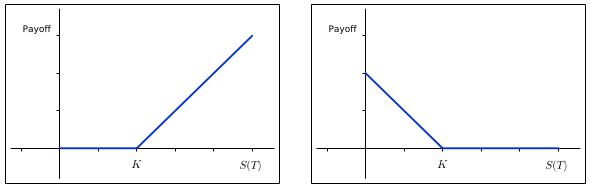
\includegraphics[width=10cm]{payofflong}
      %\caption{Payoff de posiciones long en una call y en una put con strike $K$ y madurez T.}
      \label{longpayoff}
    \end{figure}

    \begin{figure}[H]
      \centering
      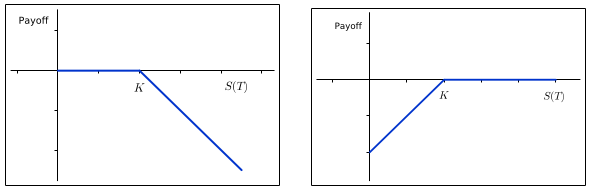
\includegraphics[width=10cm]{payoffshort}
      %\caption{Payoff de posiciones short en una call y en una put con strike $K$ y madurez T.}
      \label{shortpayoff}
    \end{figure}

  \end{block}
\end{frame}



\begin{frame}{Introducci\'on}

    \begin{block}{Ganancia.}

    El beneficio o ganancia real del inversor es el payoff mas el costo de la prima 
    
    \centerline{Payoff $\pm$ prima}

    donde $\pm$ depender\'a de la posici\'on long $(-)$ o la posici\'on short $(+)$

    \end{block}


\end{frame}

\begin{frame}{Introducci\'on}

    \begin{block}{Ganancia.}

    \begin{figure}[]
       \centering
       \begin{minipage}[b]{0.45\textwidth}
        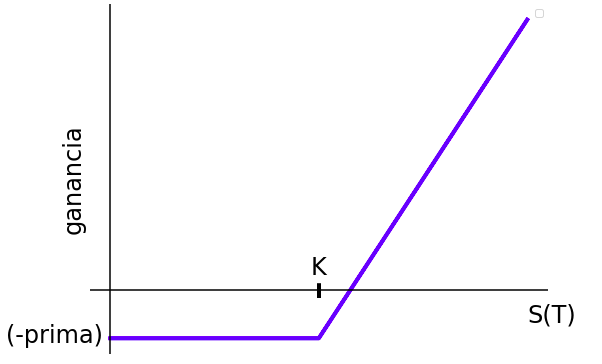
\includegraphics[width=1\textwidth]{callganancia.png}  
       \end{minipage}
       \hfill
       \begin{minipage}[b]{0.45\textwidth}
        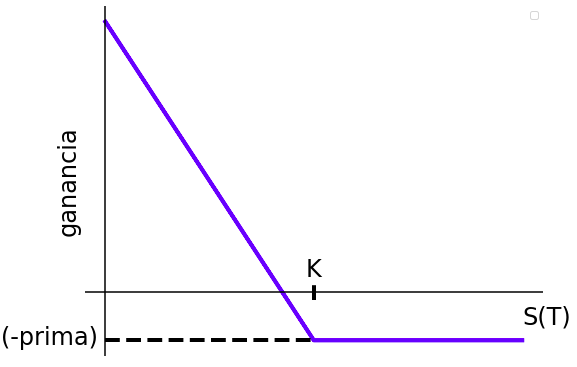
\includegraphics[width=1\textwidth]{putganancia.png}
      \end{minipage}
      %\caption{Ganancia de posiciones long en una call y en una put con strike $K$ y madurez $T$.}
      \label{longganancia}
    \end{figure}


    \begin{figure}[]
    \centering
    \begin{minipage}[b]{0.45\textwidth}
      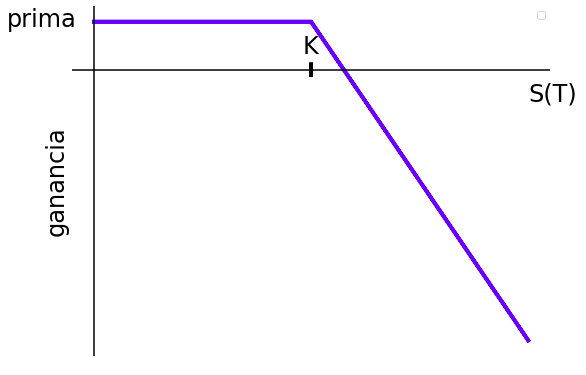
\includegraphics[width=1\textwidth]{callshorty.png}  
    \end{minipage}
    \hfill
    \begin{minipage}[b]{0.45\textwidth}
      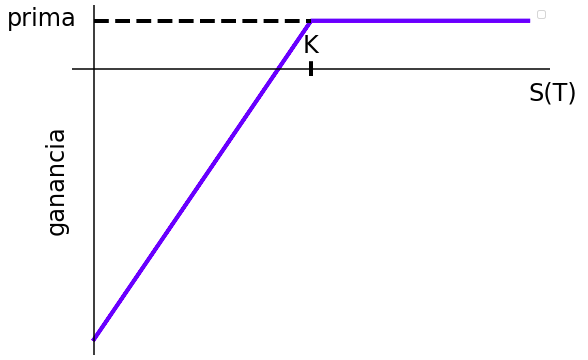
\includegraphics[width=1\textwidth]{putshorty.png}
    \end{minipage}
    %\caption{Ganancia de posiciones short en una call y en una put con strike $K$ y madurez $T$.}
    \label{shortganancia}
    \end{figure}


  \end{block}

\end{frame}

\begin{frame}{Introducci\'on}

    \begin{block}{Estrategias.}

    Las estrategias son mecanismos que utilizan los inversionistas para obtener ganancia,
    o cubrirse de posibles casos adversos.

    \begin{itemize}
        \item \textbf{Spreads}: Los \textit{spreads} son estrategias que utilizan opciones del mismo tipo (todas call o todas put).
        \item \textbf{Combinaciones}: Las \textit{combinaciones}, son estrategias que consisten en posiciones en distintos tipos de opci\'on, tanto call como puts.
    \end{itemize}    

    \end{block}

\end{frame}

\begin{frame}{Introducci\'on}

    \begin{block}{F\'ormula de Black Scholes.}

    Sea c la prima de una opci\'on call europea, con strike K, r la tasa libre de riesgo, madurez T y con precio del subyacente $S(0)$,
    sobre un activo cuyo precio sigue un movimiento geom\'etrico browniano con tendencia $r$ y
    volatilidad $\sigma$ bajo las probabilidades de riesgo neutral.
    Entonces, bajo una hip\'otesis de no arbitraje se cumple que:


    \begin{equation}
    c = S(0)\Phi(d_1) - Ke^{-rT}\Phi(d_2)
    \end{equation}

    donde:

    $\Phi$ es la distribuci\'on normal est\'andar acumulada.

    $d_1 = \displaystyle\frac{Log \left(\displaystyle\frac{S(0)}{K}\right)+ 
    \left( r + \displaystyle\frac{\sigma^2}{2}\right)T}{\sigma\sqrt{T}}$
    \qquad  $d_2 = d_1 - \sigma\sqrt{T}$


    \end{block}

\end{frame}

\begin{frame}{Introducci\'on}

    \begin{block}{Volatilidad Hist\'orica}

    La volatilidad hist\'orica como su nombre lo indica muestra el riesgo hist\'orico
    de un periodo de tiempo de hoy hacia atr\'as. Se calcula midiendo las variaciones
    que han tenido los rendimiento del activo en cierto periodo de tiempo.

    \begin{eqnarray}
      x_t = \ln \left(\displaystyle\frac{S_t}{S_{t-1}}\right)
      \\
      \overline{X} = \displaystyle\frac{1}{n}\sum_{t=1}^{n} x_t
    \end{eqnarray}

    \begin{equation}
      \label{histo}
      \mbox{Volatilidad Historica} =\frac 1{\Delta t}\cdot  \sqrt{\displaystyle\frac{1}{n-1}\sum_{t=1}^{n} (x_t -\overline{X})^2} 
    \end{equation}

    \end{block}

\end{frame}

\begin{frame}{Introducci\'on}

    \begin{block}{Volatilidad Impl\'icita}

    La volatilidad impl\'icita muestra cual es el riesgo que est\'an percibiendo los
    inversionistas de hoy en adelante, al contrario de la volatilidad hist\'orica, esta
    es una volatilidad futura. Es calculada midiendo impl\'icitamente como se
    est\'an valorando o a que precios se est\'an vendiendo los contratos de opciones
    de cierto activo.

    \end{block}

\end{frame}




\begin{frame}{Introducci\'on}

  \begin{block}{Superficie de Volatilidad}
    Una superficie de volatilidad es una representaci\'on tridimensional de las volatilidades
    impl\'icitas de un subyacente en relaci\'on con los diferentes precios de ejercicio y las
    diferentes fechas de madurez.
  \end{block}

  \begin{table}[]
    \centering
    \begin{tabular}{l|lllll}
                 & \multicolumn{5}{c}{$K/S_0$} \\ \cline{2-6}

                          & $0.9$  & $0.95$ & $1.00$ & $1.05$ & $1.10$ \\ \cline{2-6}
                $1$ mes   & $14.2$ & $13.0$ & $12.0$ & $13.1$ & $14.5$ \\ 
                $3$ meses & $14.0$ & $13.0$ & $12.0$ & $13.1$ & $14.2$ \\ 
                $6$ meses & $14.1$ & $13.3$ & $12.5$ & $13.4$ & $14.3$ \\ 
                $1$ a\~no   & $14.7$ & $14.0$ & $13.5$ & $14.0$ & $15.1$ \\ 
                $2$ a\~nos  & $15.0$ & $14.4$ & $14.0$ & $14.5$ & $15.1$ \\ 
                $5$ a\~nos  & $14.8$ & $14.6$ & $14.4$ & $14.7$ & $15.0$ \\ 
    \end{tabular}
  \end{table}

\end{frame}


\begin{frame}{Introducci\'on}

    \begin{block}{M\'etodo de Bisecci\'on}

    El m\'etodo de bisecci\'on se basa en el teorema de valor intermedio para f
    funci\'on continua. Si f es continua en el intervalo [a,b] y $f(a)f(b)< 0$, entonces
    f tiene al menos una ra\'iz en (a,b).

    \end{block}

    \begin{block}{M\'etodo de Brent}

    El m\'etodo de Brent es un algoritmo de b\'usqueda de ra\'ices que combina el
    m\'etodo de bisecci\'on, el m\'etodo secante y la interpolaci\'on cuadr\'atica inversa.

    \end{block}

\end{frame}

\begin{frame}{Introducci\'on}

  \begin{block}{Perceptr\'on}
    La unidad b\'asica de una red neuronal son los perceptrones (o neuronas). Un
    perceptr\'on toma un vector de entradas de valor real, calcula la combinaci\'on
    lineal de estas entradas con respecto a los pesos, luego genera una salida. Mas precisamente:
    $o(x_1,...,x_n) = \psi(w_0+x_1w_1+...+x_nw_n)$
  \end{block}
    
  \begin{figure}
      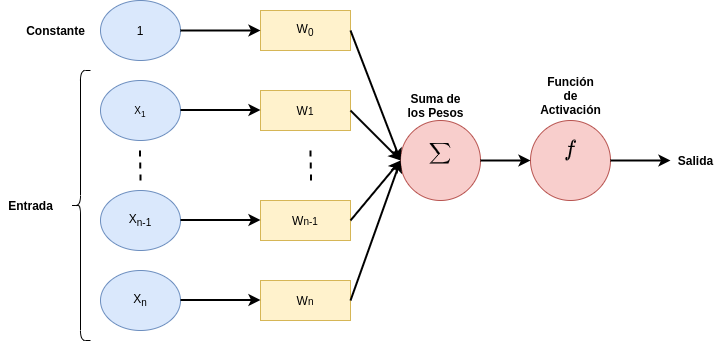
\includegraphics[scale=0.35]{perceptron}
      %\caption{Percentr\'on}
  \end{figure}
    
\end{frame}

\begin{frame}{Introducci\'on}

  \begin{block}{Red Feed-Forward}
    Este tipo de algoritmo recibe el nombre de red porque se construye componiendo funciones (perceptrones).
  \end{block}

  \begin{figure}
      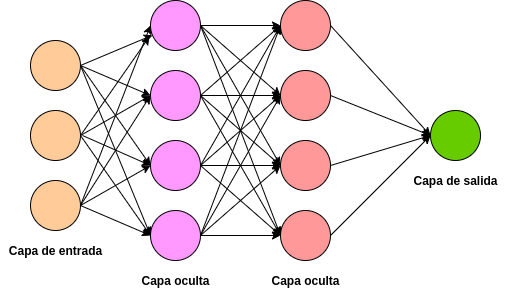
\includegraphics[scale=0.5]{feedforward}
      %\caption{Redes Feed-Forward}
  \end{figure}
  
\end{frame}



\begin{frame}{Introducci\'on}

  \begin{block}{Descenso por el Gradiente}
    El objetivo de una red neuronal es estimar los par\'ametros \'optimos para una funci\'on $f(x,W,b)$. Una forma de estimar esos par\'ametros es reducir el error. Sea 

    $J(x,W,b,Y) = \displaystyle\frac{1}{n}\sum\limits_{i=1}^{n}(f(x_i,W,b) - y_i)^2$ 

    una funci\'on de costo.
  \end{block}
  
  \begin{figure}
      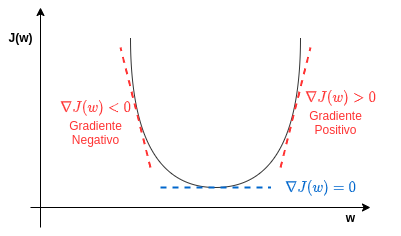
\includegraphics[scale=0.4]{funcion_costo}
      %\caption{Aprendizaje por Descenso del Gradiente}
  \end{figure}

\end{frame}



\begin{frame}{Introducci\'on}

  \begin{block}{Funci\'on de activaci\'on}
    La funci\'on de activaci\'on en las redes neuronales son las encargadas de
    enviar se\~nales al siguiente nivel o siguiente capa.
  \end{block}
  
  \begin{eqnarray}
    ReLu(z) = \max(z,0) 
    \label{Relu} 
    \\
    \tanh(z) = \displaystyle\frac{e^z - e^{-z}}{e^z + e^{-z}} %latex fuction buscar
    \label{Tanh} 
    \\
    Elu(z)= \begin{cases}
              \alpha(e^{z -1}) & \mbox{si } z < 0\\
              z  &   \mbox{si }z \ge 0
            \end{cases}
  \label{Elu}
  \end{eqnarray}
            

\end{frame}



\begin{frame}{Introducci\'on}

  \begin{block}{Tasa de aprendizaje}
    La tasa de aprendizaje determina el tama\~no del paso en cada iteraci\'on mientras se
    mueve hacia un m\'inimo de una funci\'on de error.
  \end{block}
  \begin{figure}
      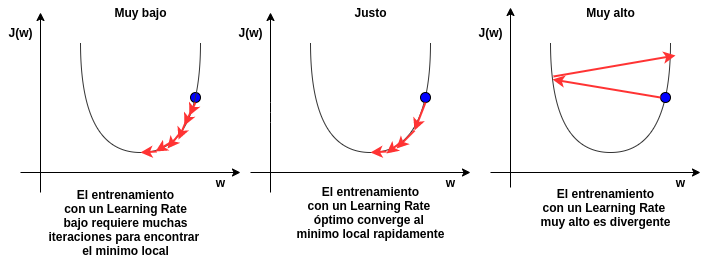
\includegraphics[scale=0.45]{learning_rate}
      %\caption{Learning Rate}
  \end{figure}

\end{frame}



\begin{frame}{Introducci\'on}

  \begin{block}{Tasa de aprendizaje c\'iclico}

  En este caso la tasa de aprendizaje var\'ia entre un m\'inimo y m\'aximo, creciendo y decreciendo.

  \end{block}

  \begin{figure}
    \centering
    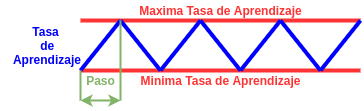
\includegraphics[width=0.8\textwidth%12cm, height=4cm
    ]{cyclical_lr.png}
  \end{figure}

\end{frame}



\begin{frame}{Introducci\'on}


   \begin{block}{k-fold cross validation}

        K-fold cross validation es una t\'ecnica utilizada para evaluar modelos propuestos, con el fin de
        encontrar el mejor modelo.

    \end{block}

\end{frame}


\begin{frame}{Superficie de volatilidad para valorar opciones}

  \begin{block}{Modelos para valoraci\'on de opciones}
  Para valorar las opciones existen modelos matem\'aticos.
  \end{block}
    \begin{itemize}
      \item Black-Scholes (1973): Modelo para valorar opciones europeas.
      \item Rubinstein (1991): Modelo para valorar opciones chooser simples.
      \item Conze y Viswanathan (1991): Modelo para valorar opciones lookbacks con precio de ejercicio fijo.
      \item Goldman, Sosin y Gatto (1979): Modelo para valorar opciones lookbacks con precio de ejercicio flotante.
      \item Kemma y Vorst (1990): Modelo para valorar opciones asi\'aticas con media geom\'etrica.
      \item Levy (1992): Modelo para valorar opciones asi\'aticas con media aritm\'etica.
      \item Margrabe (1978): Modelo para valorar opciones sobre el intercambio de dos activos.
    \end{itemize}


\end{frame}


\begin{frame}{Estrategias}


   \begin{block}{Backspread}

        \begin{itemize}

            \item El inversor espera un movimiento particular del mercado, pero teniendo un poco de protecci\'on en caso de equivocarse.
            \item Busca que la volatilidad impl\'icita sea baja al momento de aplicar la estrategia, con esperanza que suba en el futuro.

        \end{itemize}

    \end{block}

\end{frame}

\begin{frame}{Estrategias}


   \begin{block}{Backspread}

   \begin{figure}
            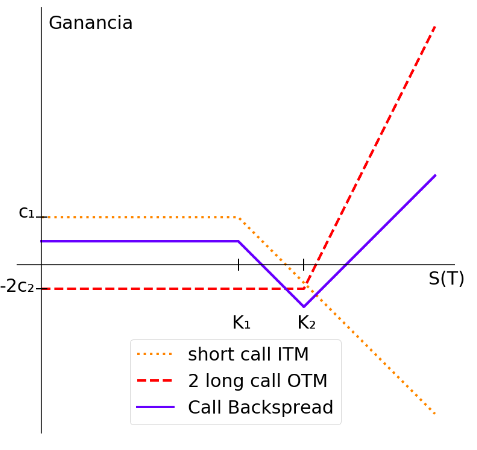
\includegraphics[width=0.475\textwidth]{backspread}
            \hfill
            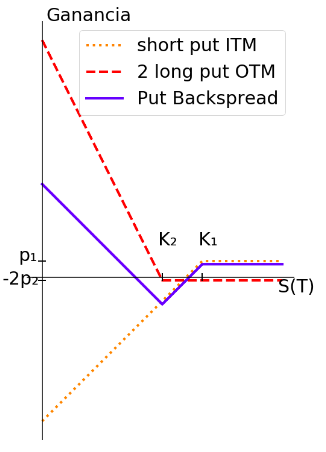
\includegraphics[width=0.475\textwidth]{backspreadput}
        \end{figure}

    \end{block}

\end{frame}

\begin{frame}{Estrategias}

    \begin{block}{Long Straddle o Long Strangle}

      \begin{itemize}
        \item El inversor tiene expectativa que el valor del subyacente tenga un gran cambio, sin importar si el precio sube o baja.
        \item Se busca que la volatilidad impl\'icita sea baja al momento de aplicar la estrategia.
        \item Idealmente se busca opciones out-of-the-money. 
        \item Se busca que sean opciones largas.%para que el precio del subyacente varie lo suficiente
      \end{itemize}


    \end{block}

\end{frame}

\begin{frame}{Estrategias}

    \begin{block}{Long Straddle}

        \begin{figure}
            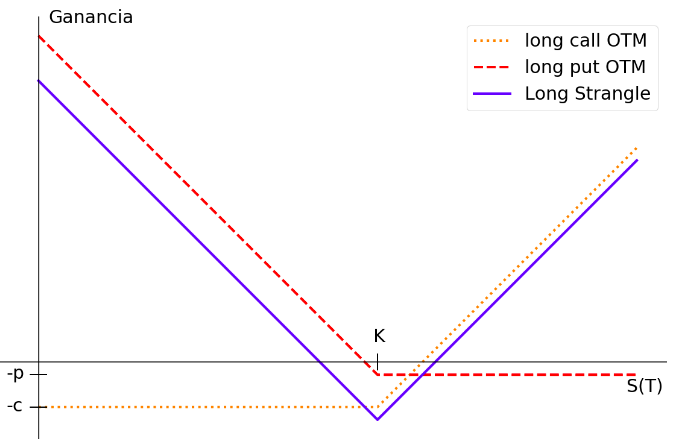
\includegraphics[scale=0.45]{straddle}
        \end{figure}

    \end{block}

\end{frame}

\begin{frame}{Estrategias}

    \begin{block}{Long Strangle}

        \begin{figure}
            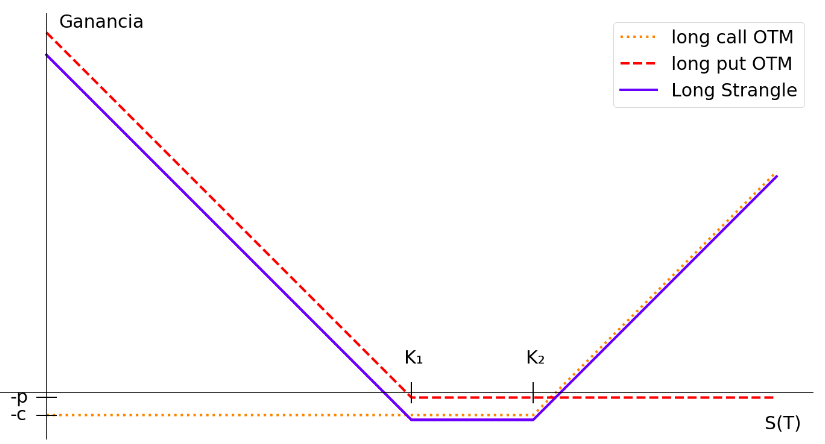
\includegraphics[scale=0.37]{strangle}
        \end{figure}

    \end{block}

\end{frame}


\begin{frame}{Estrategias}

    \begin{block}{Long Butterfly Spread}

        \begin{itemize}

            \item El inversor tiene expectativa que el valor del subyacente no var\'ie mucho hasta su vencimiento.
            \item Se busca que la volatilidad impl\'icita sea alta al momento de aplicar la estrategia, cu\'anto m\'as alta mejor.
            \item Se invierte en opciones cortas, con un tiempo de expiraci\'on menor a 60 d\'ias.


        \end{itemize}
    \end{block}

\end{frame}



\begin{frame}{Estrategias}

    \begin{block}{Long Butterfly Spread}

        \begin{figure}
            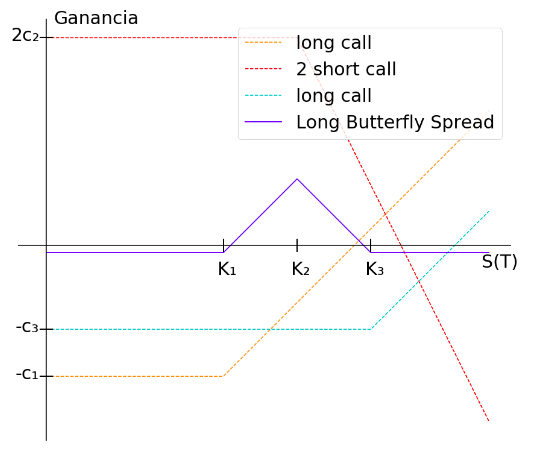
\includegraphics[scale=0.45]{butterfly}
        \end{figure}

    \end{block}

\end{frame}


\begin{frame}{M\'etodos Num\'ericos}

    
    \begin{itemize}[<+->]
        \item Funci\'on a aplicar.
        \item g es mon\'otona creciente con respecto a $\sigma$
        \item Inicializaci\'on de intervalo para m\'etodo
              de bisecci\'on y de brent
        \item Aplicaci\'on de los m\'etodos
        
    \end{itemize}

    \begin{block}{Procedimiento}
        \only<1>{\begin{equation}
                    g(\hat{\sigma}) = S(0)\Phi(d_1) - Ke^{-rT}\Phi(d_2) - c
                \end{equation}

                donde:

                c es la prima de la call europea y el resto de las variables definidas en (1)

                $\Phi$ es la distribuci\'on normal est\'andar acumulada.

                $d_1 = \displaystyle\frac{Log \left(\displaystyle\frac{S(0)}{K}\right)+ 
                \left( r + \displaystyle\frac{\hat{\sigma}^2}{2}\right)T}{\hat{\sigma}\sqrt{T}}$
                \qquad  $d_2 = d_1 - \hat{\sigma}\sqrt{T}$
        }
        \only<2>{Sabemos que f\'ormula de Black Scholes es mon\'otona creciente con respecto a $\sigma$,
                entonces g tambien es creciente con respecto a $\sigma$
        }
        \only<3>{Buscamos [a, b] talque $f(a)f(b) < 0$}
        \only<4>{Aplicamos bisecci\'on y brent utilizando g, sobre [a,b], hasta encontrar la ra\'iz o
                 cumplir con una cierta tolerancia.
        }

    \end{block}

\end{frame}


\begin{frame}{M\'etricas}
  \begin{eqnarray}
  \mbox{ECM} &=& \frac{1}{N} \sum_{i=1}^{N}(y_i - \hat{y_i})^2 \label{eq:ECM}
  \\
  \mbox{EAM} &=& \frac{1}{N} \sum_{i=1}^{N}|y_i - \hat{y_i}| 
  \\
  \mbox{EPAM} &=& 100 \frac{1}{N} \sum_{i=1}^{N}\displaystyle\frac{|y_i - \hat{y_i}|}{y_i} \label{eq:EPAM}
%  \\
 % \overline{y} = \displaystyle\frac{1}{N}\sum_{i=1}^{N} y_i 
  \\
  SS_{tot} &=& \sum_{i=1}^{N} (y_i-\overline{y})^2 ,\qquad \mbox{ con }  \overline{y} = \frac{1}{N}\sum_{i=1}^{N} y_i 
  \\
  R^2 &=& 1 - \frac{\mbox{ECM}}{SS_{tot}} \label{eq:Rcuad}
\end{eqnarray}
\end{frame}


\begin{frame}{Redes Neuronales}

    \begin{block}{C\'alculo de prima de opci\'on call con ratio}
        
        Rene Garcia y Ramazan Gen\c{c}ay, invocando la homogeneidad de la f\'ormula de Black-Scholes,
        demostraron que las redes neuronales estiman mejor el precio de una opci\'on usando el cociente $S/K$.

        \begin{eqnarray}
            \frac{c}{K} &=& \frac{B(S(0),K,r,\sigma,T)}{K}\\
            & =& \frac{S(0)}{K}\Phi\left(d_1\left(\frac {S(0)}K\right)\right) - e^{-rT}\Phi\left(d_2\left(\frac {S(0)}K\right)\right)\\
              & =& \tilde B\left(\frac{S(0)}K, T, r, \sigma\right)\notag
            \label{c2}
        \end{eqnarray}
%
        donde $d_1$, $d_2$ y $\Phi$ son las funciones definidas anteriormente.


    \end{block}

\end{frame}

\begin{frame}{Redes Neuronales}

  Generaci\'on de muestra.

    \begin{table}[!htbp]
        \begin{center}
        \begin{tabular}{|l|l|l|l|l|}
            \hline
             & Parametros & muestra amplia  &  muestra estrecha   \\ \hline
              & precio ratio($S_0$/K) & [0.4, 1.6] & [0.5, 1.5]   \\ \cline{2-4} 
             Entrada & Madurez($\tau$) &  [0.2, 1.1] & [0.3, 0.95]   \\ \cline{2-4} 
              & volatilidad($\sigma$) &  [0.01, 1] & [0.02, 0.9]  \\ \cline{2-4} 
              & Tasa libre de riesgo($r$) &  [0.02, 0.1] & [0.03, 0.08] \\ \hline
             Salida & Precio de Call(c/K) &  (0, 0.9) & (0, 0.73) \\ \hline
        \end{tabular}
        \end{center}
    \end{table} 

  

\end{frame}

\begin{frame}{Redes Neuronales}
    
  8-fold cross validation.

    \begin{table}[h!]
    \begin{center}


        \begin{tabular}{c|c}
        \hline

        Par\'ametros & Opciones o Rango  \\ \hline
        Capas & [1,10]    \\ 
        Neuronas & [50,1000]  \\ 
        Funci\'on de error & ECM, EAM, EPAM  \\ 
        Funci\'on de activaci\'on & ReLu, Elu, tanh  \\ 
        Inicializaci\'on de pesos & uniform, glorot\_uniform, he\_uniform  \\ 
        Algoritmo de optimizaci\'on & SGD, RMSprop, Adam  \\ 
        Dropout & [0,0.2]  \\ 
        Tama\~no de batch & [256, 2048] \\
        \hline
        \end{tabular}
    \end{center}
    \end{table}

\end{frame}


\begin{frame}{Redes Neuronales}

    Hiperp\'arametros obtenidos con cross validation.

    \begin{table}[]
    \begin{center}
    
        \begin{tabular}{c|c}
        \hline

        Par\'ametros & Opciones  \\ \hline
        Capas & 3   \\ 
        Neuronas & 950  \\  
        Funci\'on de error & ECM  \\ 
        Funci\'on de activaci\'on & ReLu  \\ 
        Inicializaci\'on de pesos &  random\_uniform \\ 
        Algoritmo de optimizaci\'on & Adam  \\ 
        Dropout & 0  \\ 
        Tama\~no de batch &  1024 \\
        \hline
        \end{tabular}
    \end{center}
    \end{table}


\end{frame}

\begin{frame}{Redes Neuronales}
    
    M\'etodo de Smith.
                            
    \begin{figure}[]
        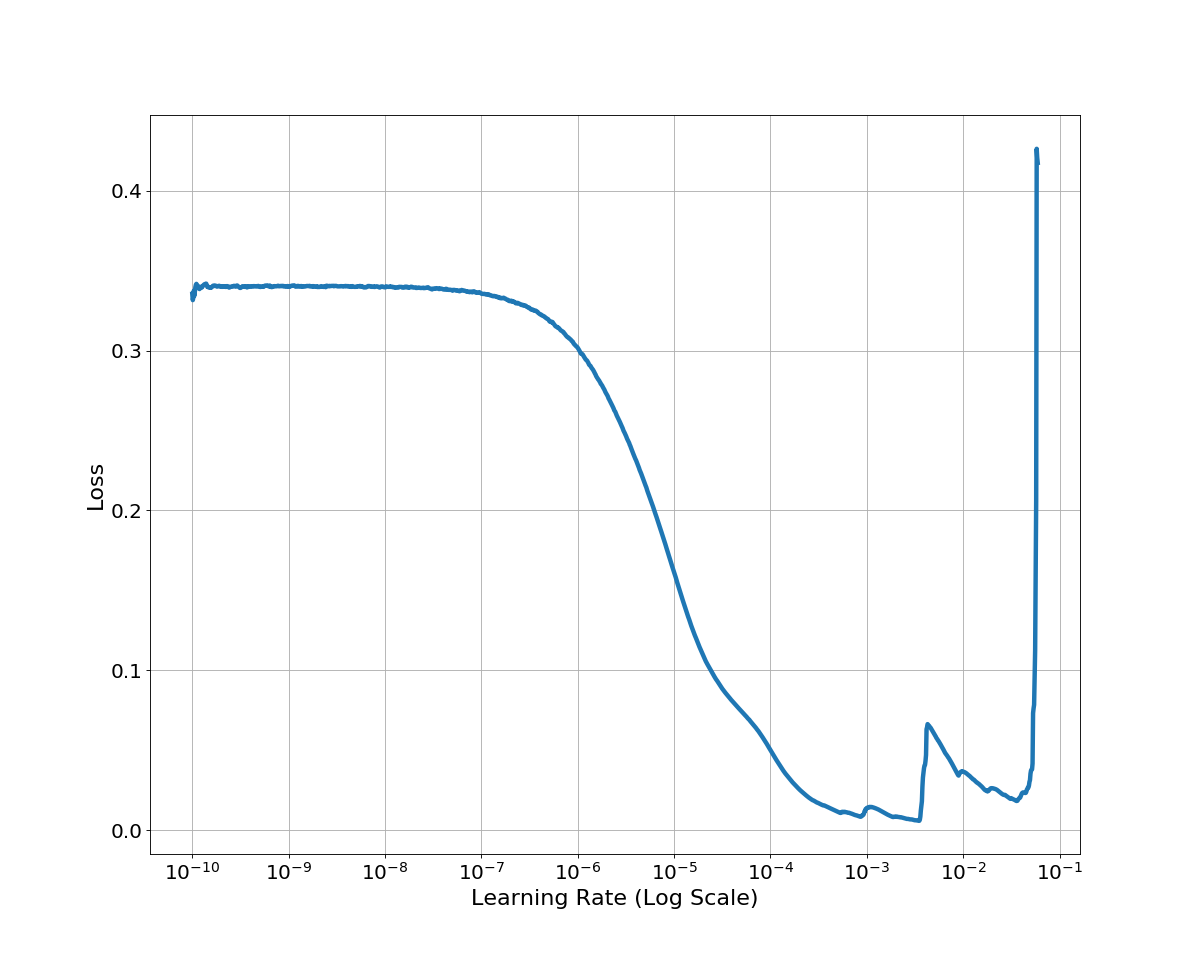
\includegraphics[scale=0.26]{learning_rate_post}
    \end{figure}


\end{frame}


\begin{frame}{Redes Neuronales}
    
    Grid-Search.
    \begin{table}[h!]
    \begin{center}
        \begin{tabular}{c|c|c|c}
        \hline

        Parametros & Step Decay & Exponential Decay  & Time-Based Decay\\ \hline
        base\_lr & [$10^{-2}$, $10^{-4}]$ & [$10^{-2}$, $10^{-4}$] & [$10^{-2}$, $10^{-4}$]\\  
        decay & [0.9, 0.95] & [0.007, 0.002] & [0.01, 8]\\ 
        epoch\_drop & [5, 50] & - & -\\ 
        \hline
        \end{tabular}
    \end{center}
    \end{table}

    Par\'ametros de los Algoritmos de Decrecimiento.
    \begin{table}[h!]
        \begin{center}
        
        \begin{tabular}{c|c|c|c}
        \hline

        Parametros & Step Decay & Exponential Decay  & Time-Based Decay\\ \hline
        base\_lr & $5*10^{-4}$ & 0.0005 & 0.005 \\  
        decay & 0.9 & 0.002 & 0.875 \\ 
        epoch\_drop & 20 & - & -\\ 
        \hline
        \end{tabular}
    \end{center}
    \end{table}

\end{frame}

\begin{frame}{Redes Neuronales}

    Comparaci\'on algoritmos de decrecimiento de la taza de aprendizaje. 
    

    \begin{figure}[!tbp]
        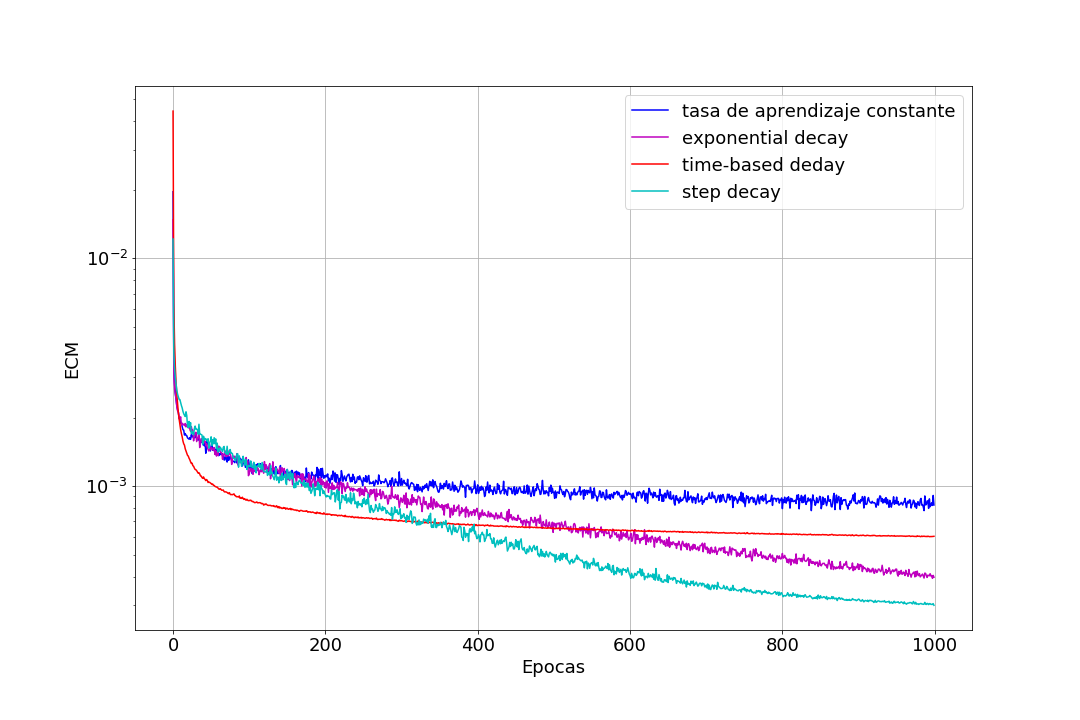
\includegraphics[scale=0.28]{comparacion_post}
    \end{figure}


\end{frame}

\begin{frame}{Redes Neuronales}

Step Decay contra Cyclical Decay.

    \begin{figure}[!tbp]
        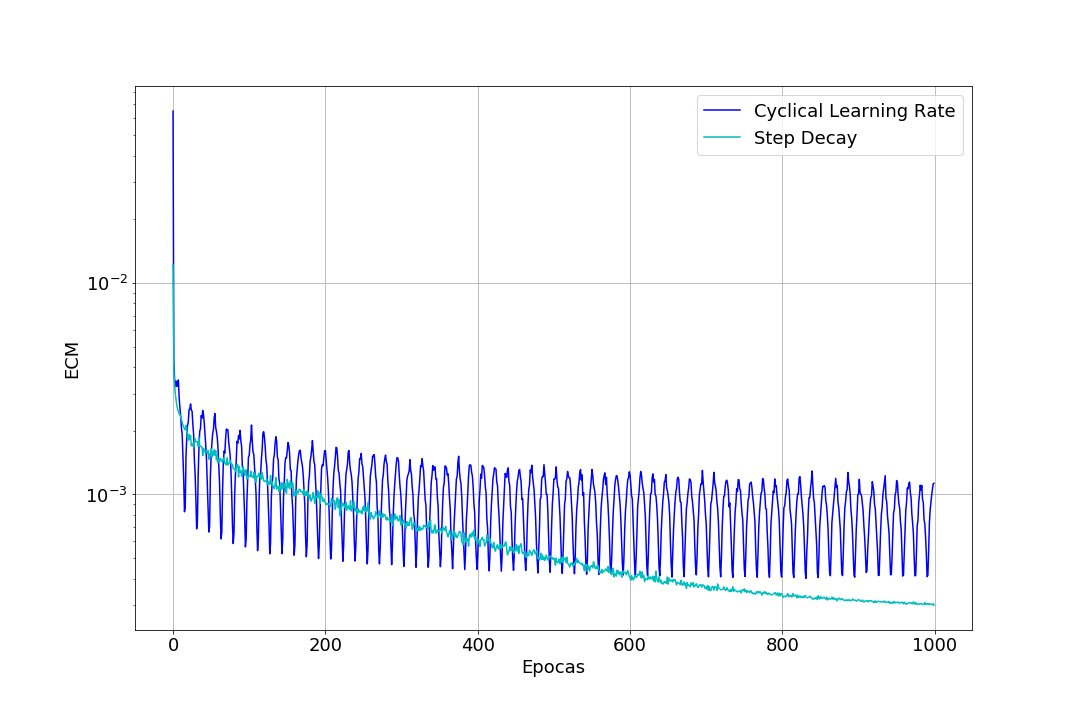
\includegraphics[scale=0.28]{step_vs_cyclical}
    \end{figure}

\end{frame}

\begin{frame}{Redes Neuronales}

    Una vez obtenidos los hiperp\'ametros y la muestra se entrenar\'a la red.

    \begin{figure}[!tbp]
      \centering
      \begin{minipage}[b]{0.45\textwidth}
        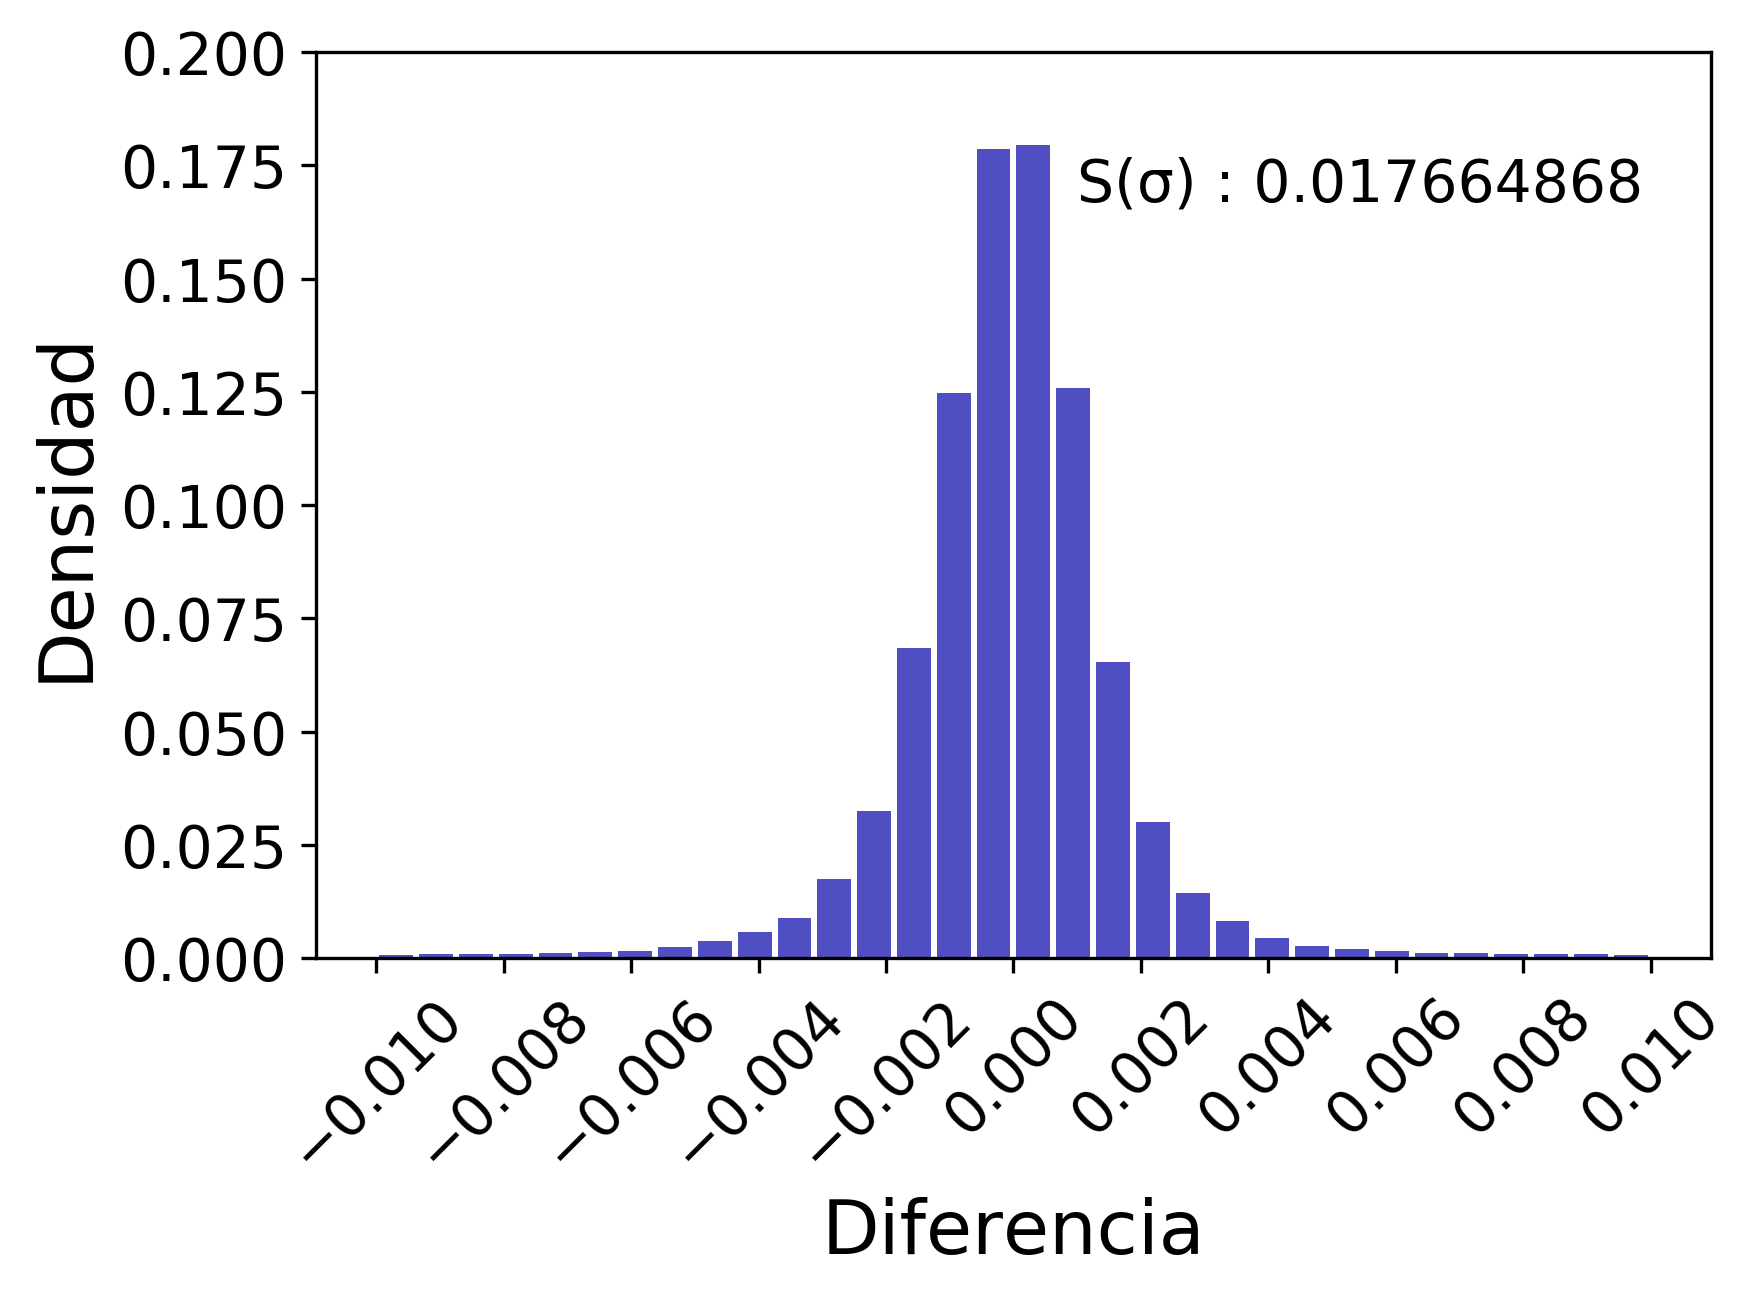
\includegraphics[width=\textwidth]{Predic_w_n.png}
        \caption{Predicci\'on muestra amplia.}
      \end{minipage}
      \hfill
      \begin{minipage}[b]{0.45\textwidth}
        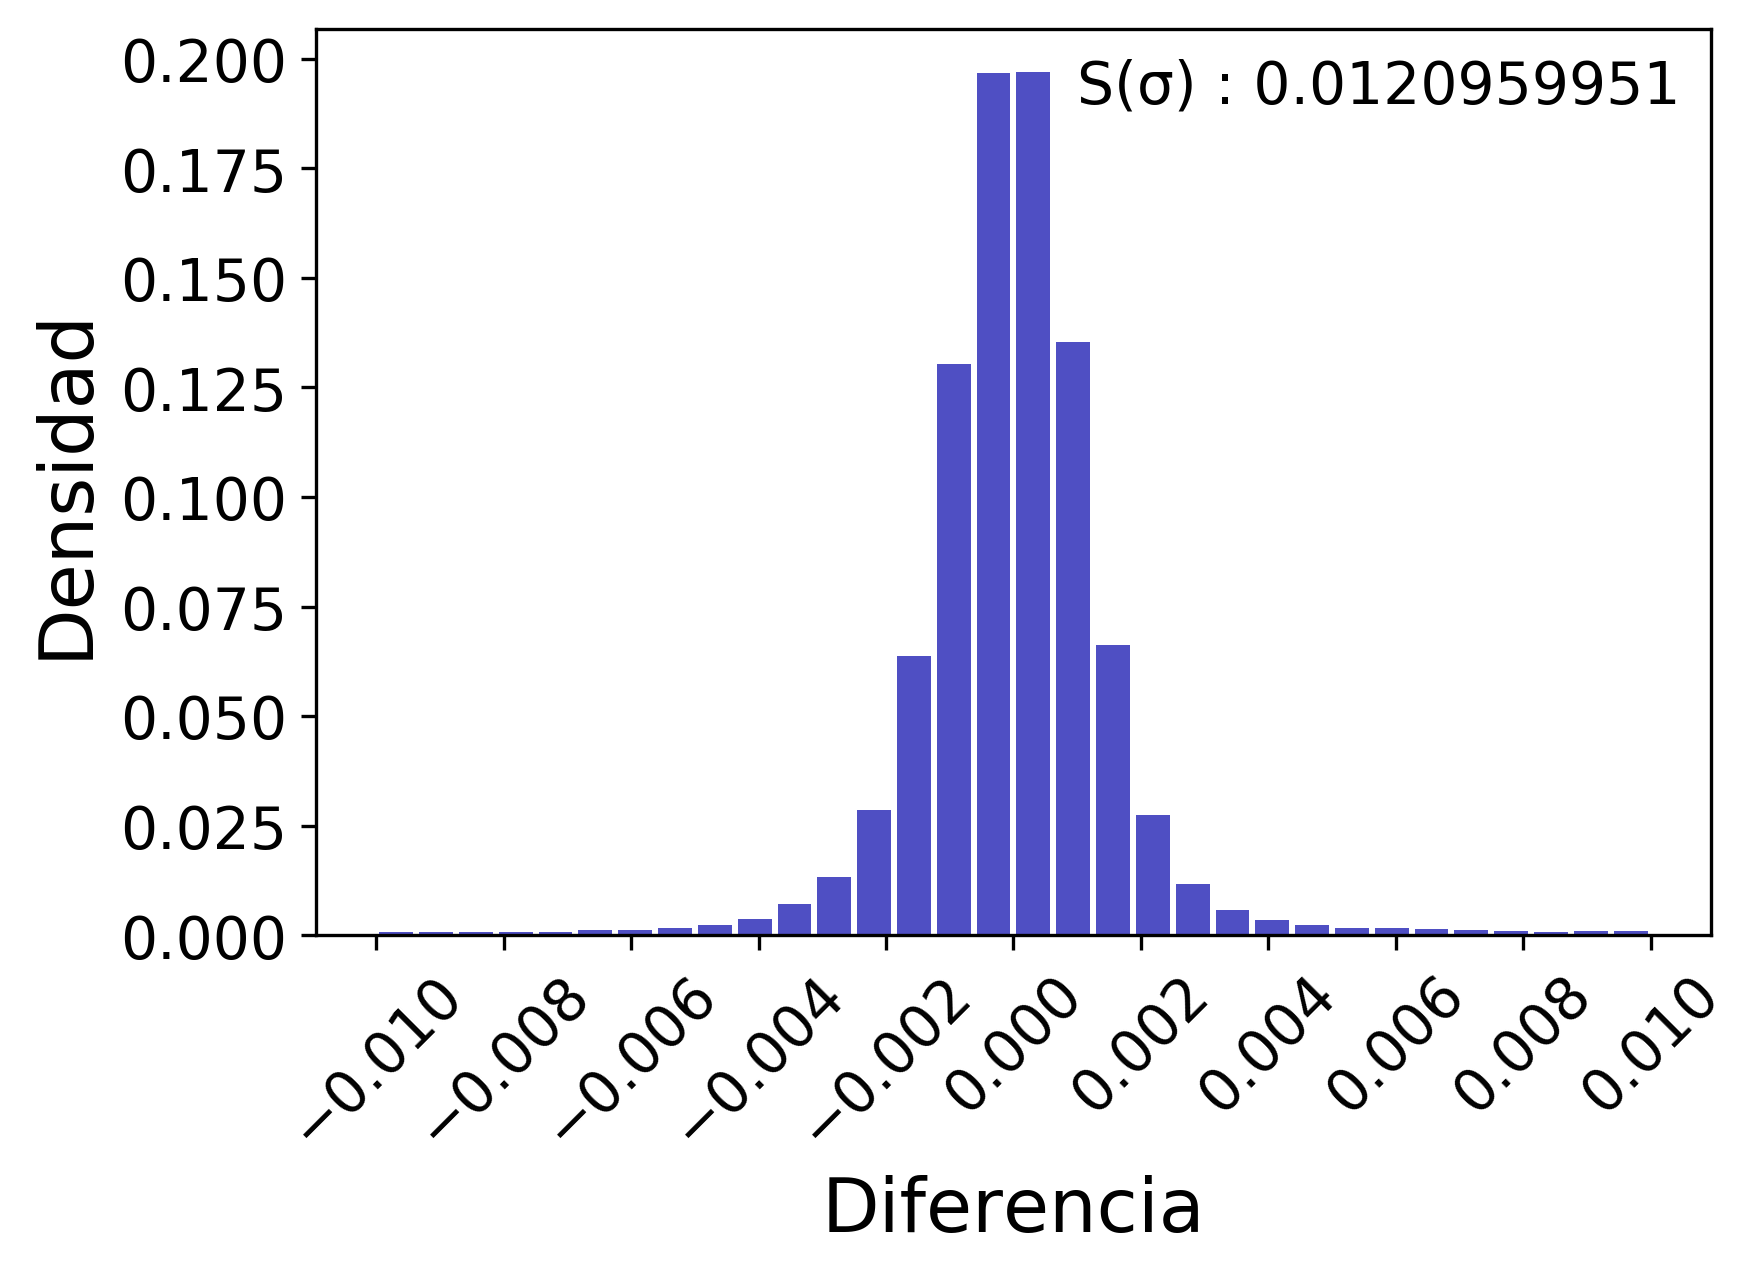
\includegraphics[width=\textwidth]{Predic_n_n.png}
        \caption{Predicci\'on muestra estrecha.}
      \end{minipage}
    \end{figure}

\end{frame}

\begin{frame}{Redes Neuronales}
    
    Sea $\tilde{C} = C - max(S_0 - Ke^{-r\tau}, 0) $

    La entrada de la red ser\'a \{log($\tilde{C}$/K), $S_0$/K, $r$, $\tau$\} y la salida \{$\sigma$\}

    \begin{figure}[!tbp]
      \centering
      \begin{minipage}[b]{0.45\textwidth}
        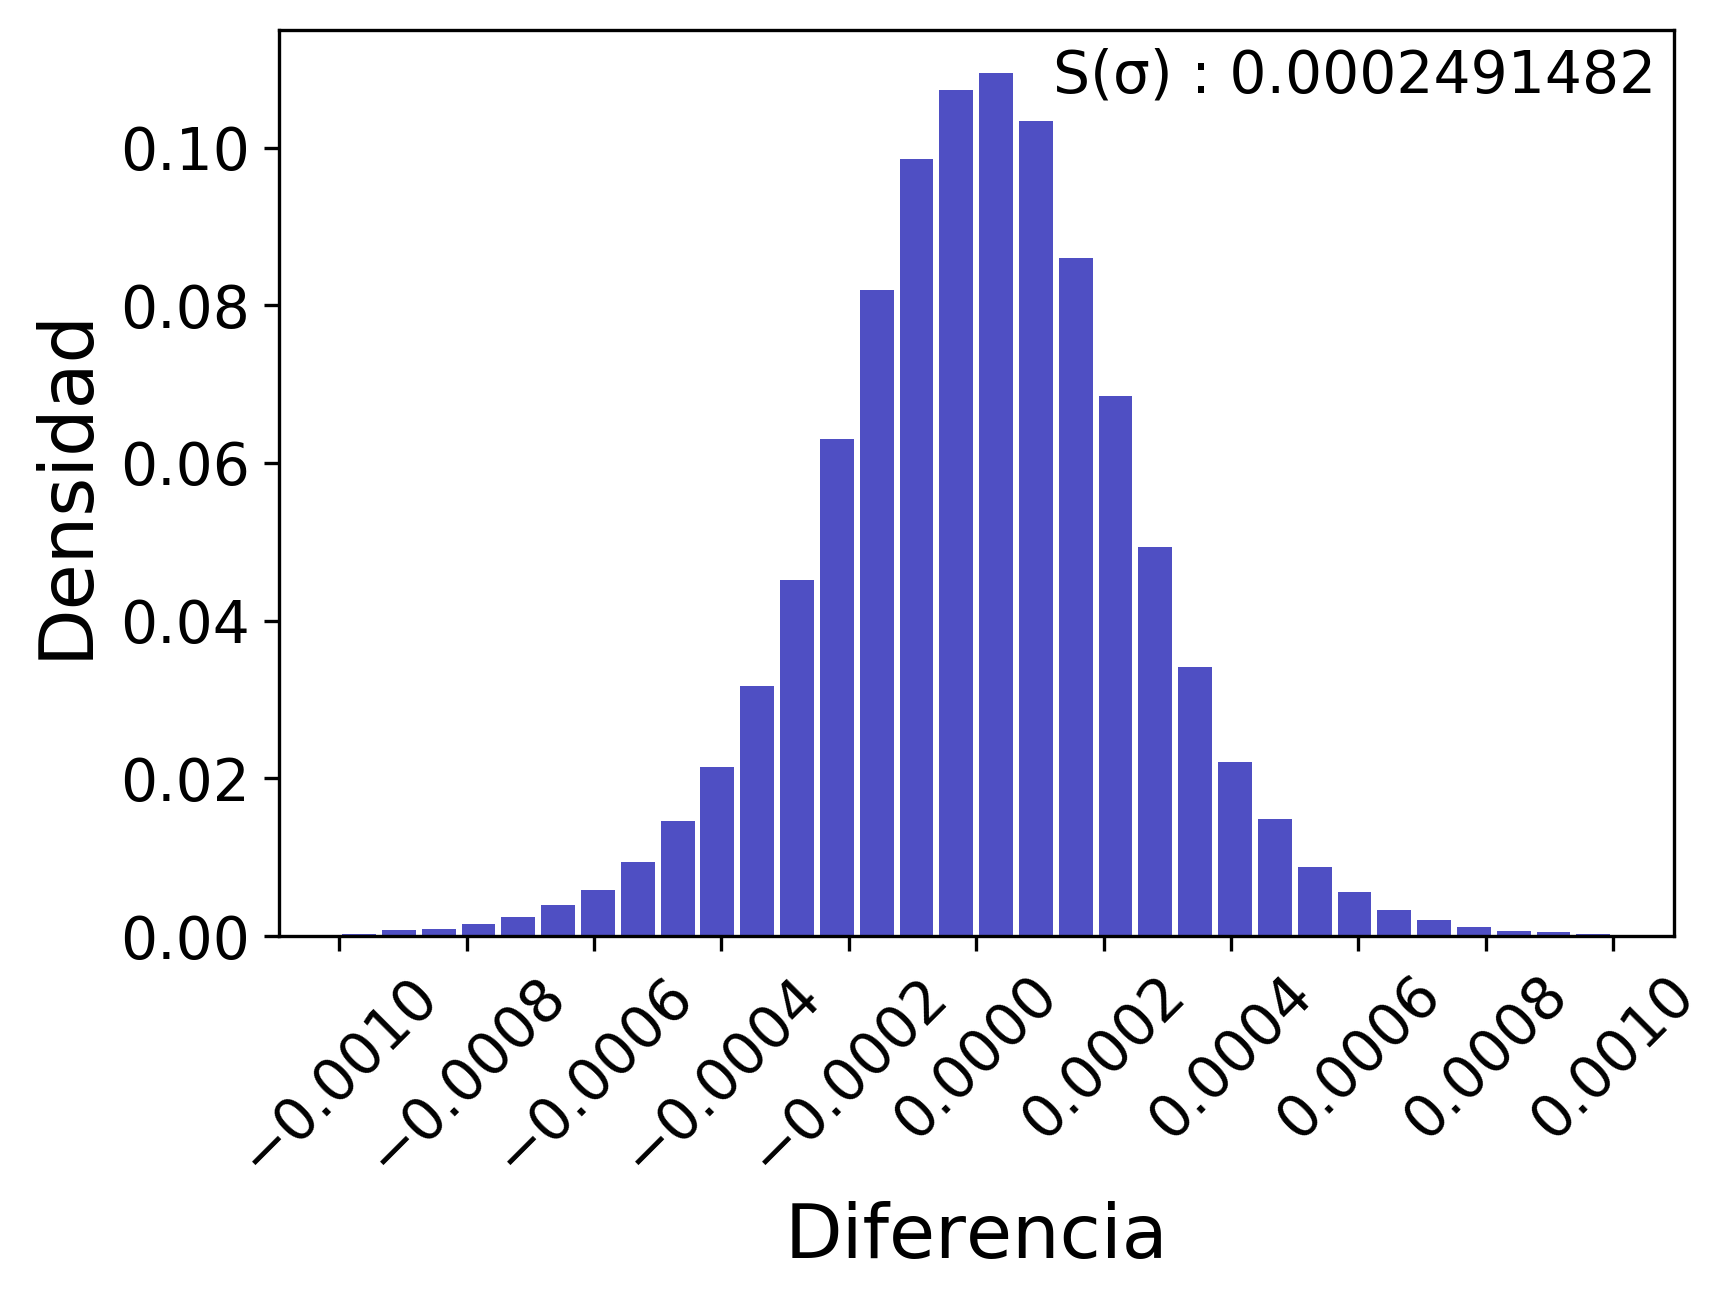
\includegraphics[width=\textwidth]{Predic_w_log_mil.png}
        \caption{Predicci\'on muestra amplia.}
      \end{minipage}
      \hfill
      \begin{minipage}[b]{0.45\textwidth}
        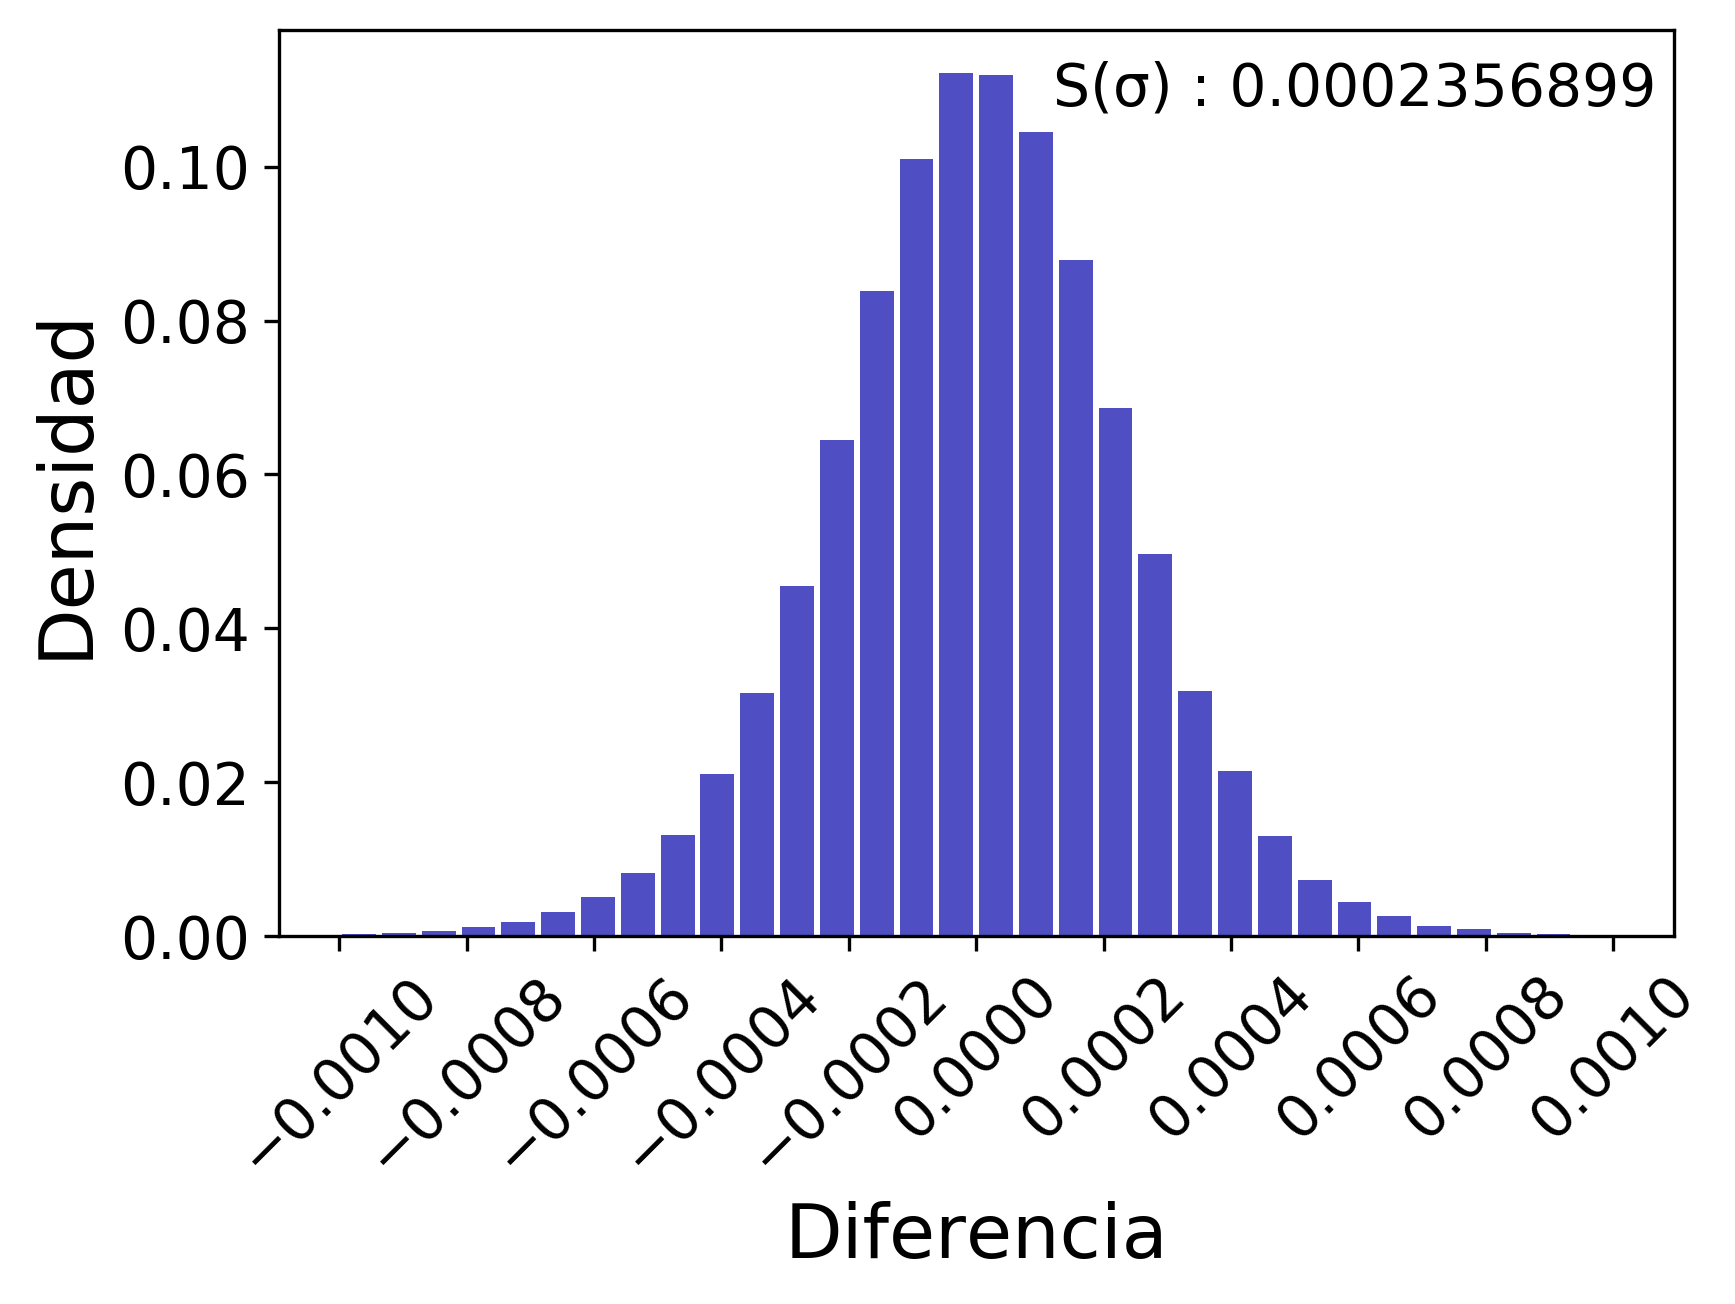
\includegraphics[width=\textwidth]{Predic_n_log_mil.png}
        \caption{Predicci\'on muestra estrecha.}
      \end{minipage}
    \end{figure}

\end{frame}

\begin{frame}{Redes Neuronales}

    \begin{figure}[!tbp]
      \centering
      \begin{minipage}[b]{0.45\textwidth}
        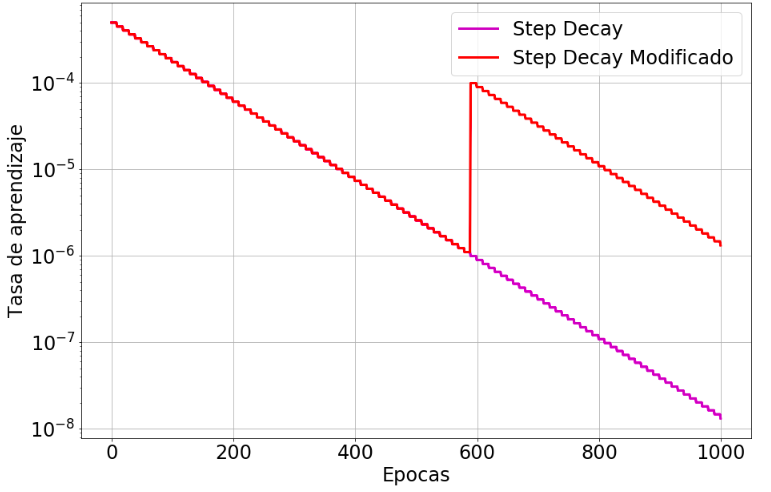
\includegraphics[width=\textwidth]{lr_1000.png}
        \caption{Learning Rate sobre 1000 epocas.}
      \end{minipage}
      \hfill
      \begin{minipage}[b]{0.45\textwidth}
        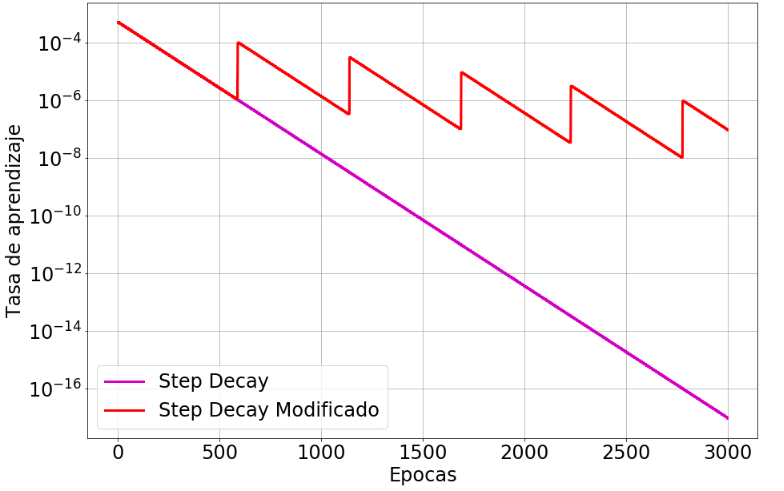
\includegraphics[width=\textwidth]{lr_3000.png}
        \caption{Learning Rate sobre 3000 epocas.}
      \end{minipage}
    \end{figure}

\end{frame}

\begin{frame}{Redes Neuronales}

  El resultado final ser\'a.
    \begin{figure}[!tbp]
      \centering
      \begin{minipage}[b]{0.45\textwidth}
        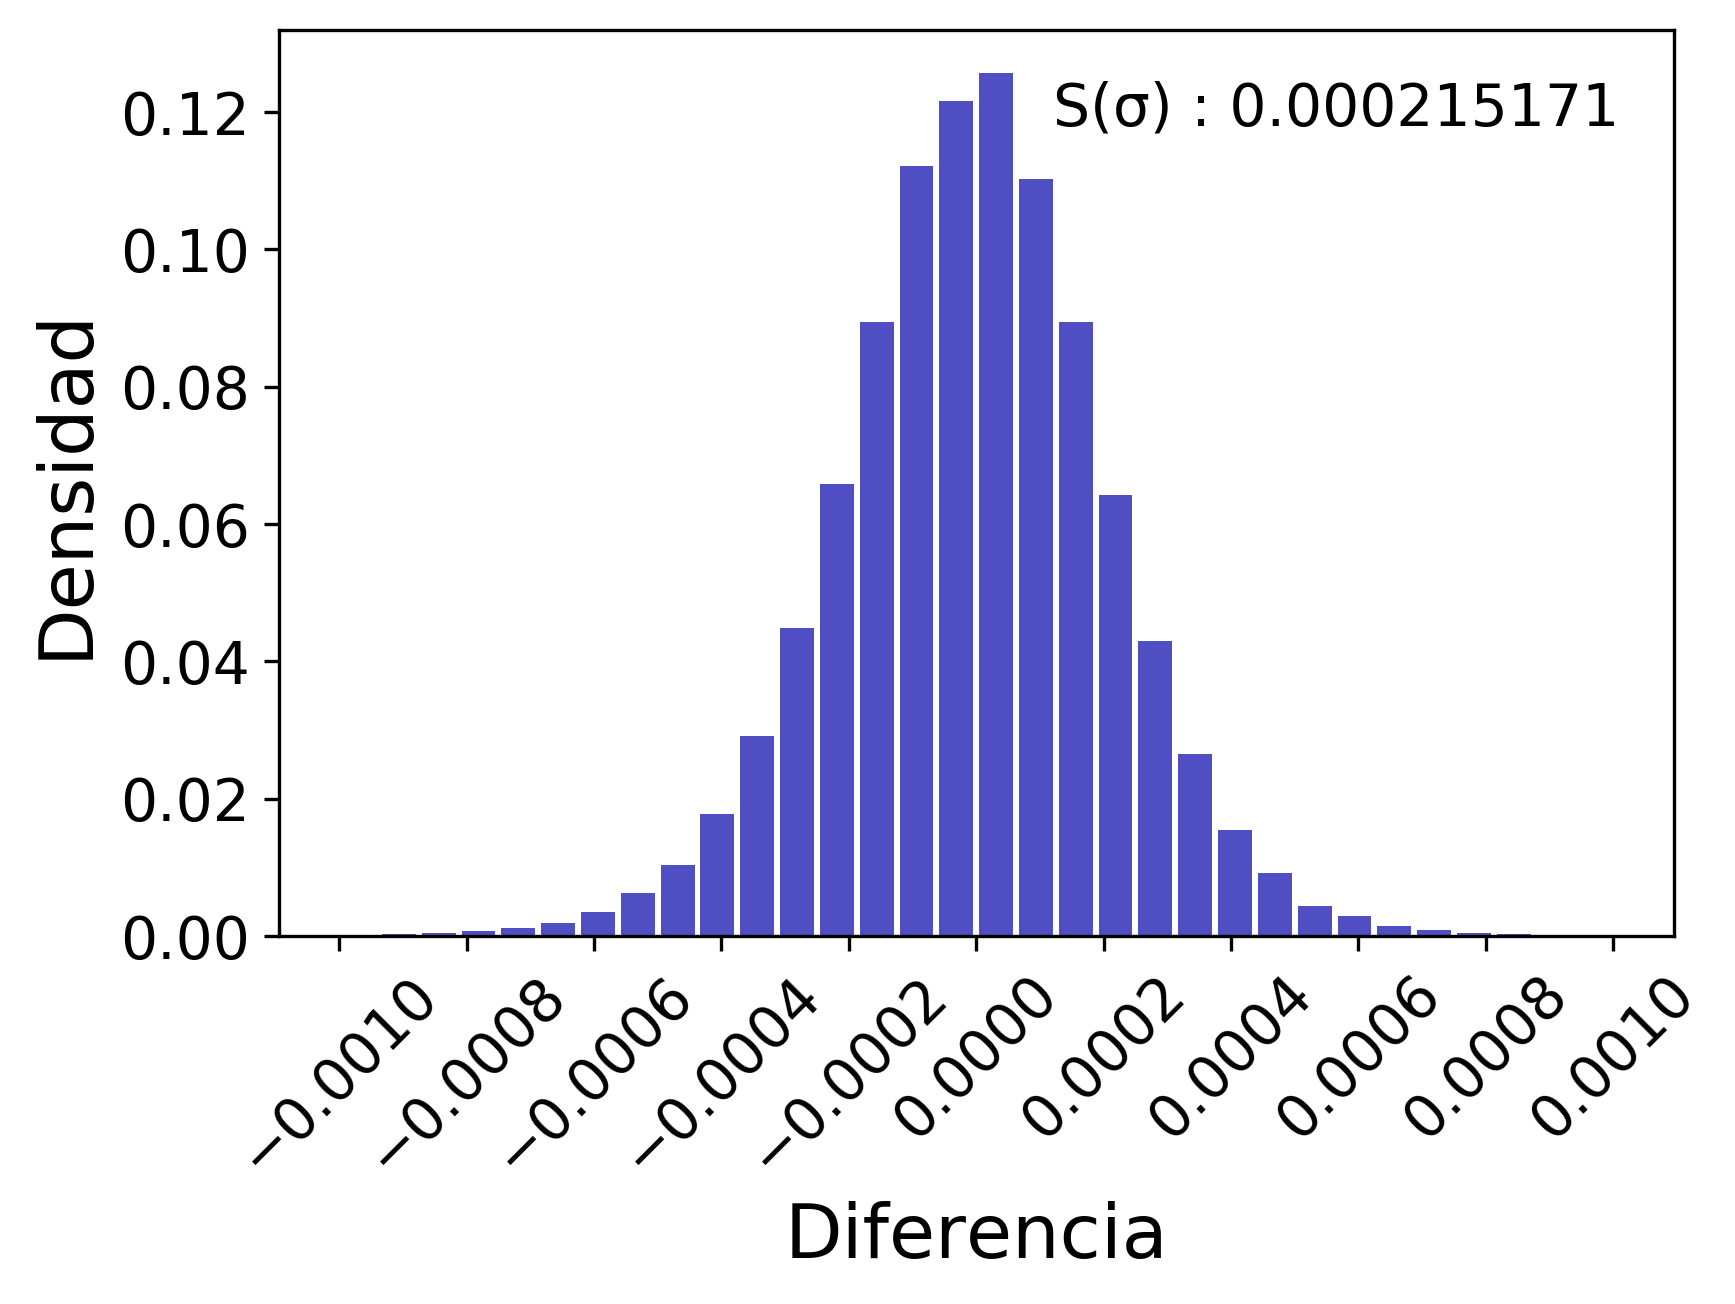
\includegraphics[width=\textwidth]{Predic_w_log_3mil.png}
        \caption{Predicci\'on muestra amplia 3000 epochs.}
      \end{minipage}
      \hfill
      \begin{minipage}[b]{0.45\textwidth}
        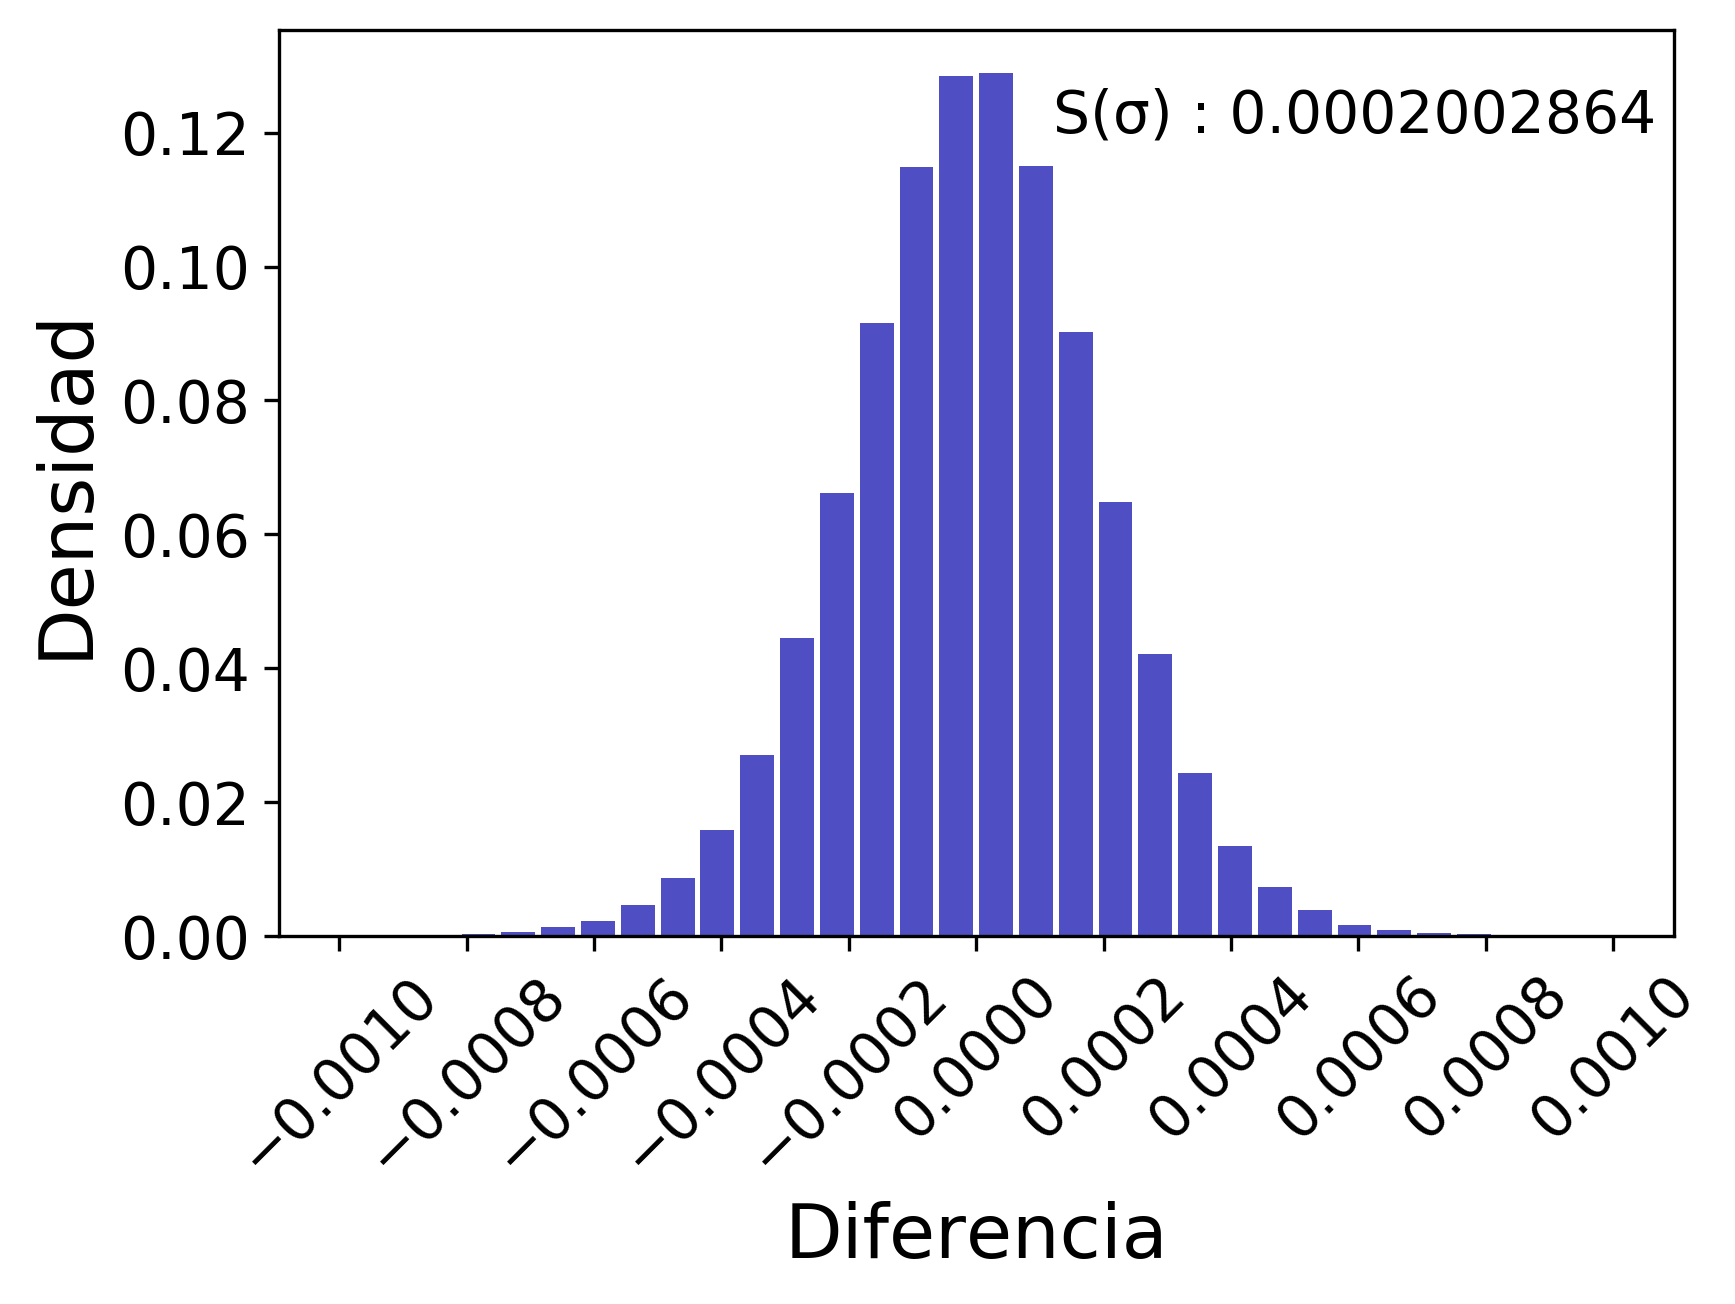
\includegraphics[width=\textwidth]{Predic_n_log_3mil.png}
        \caption{Predicci\'on muestra estrecha 3000 epochs.}
      \end{minipage}
    \end{figure} 


\end{frame}

\begin{frame}{Precisi\'on}

    Error en los modelos propuestos.
    \begin{table}[!htbp]
      \begin{center}
        \begin{tabular}{|l|l|l|l|l|}
          \hline
           & ECM & EAM  &  EPAM & $R^2$ \\ \hline
          Red inicial  & $3.21 \times 10^{-4}$ & $6.09 \times 10^{-3}$ & $9.30$ & $0.996031$ \\ \hline
          Red optimizada & $6.24\times10^{-8}$ & $1.92\times10^{-4}$ & $0.059$ & $0.999999104$ \\ \hline
          Red definitiva & $4.67\times10^{-8}$ & $1.66\times10^{-4}$ & $0.0515$ & $0.999999329$\\ \hline
          Bisecci\'on  & $1.10\times10^{-8}$ & $2.89\times10^{-6}$ & $0.00469$ & $0.99999986$  \\ \hline
          Brent & $8.17\times10^{-6}$ &  $ 9.18\times10^{-5}$ & $0.35894$ & $0.99989551$  \\ \hline
        \end{tabular}
      \end{center}
    \end{table}


\end{frame}

\begin{frame}{N\'umeros Representables}

    \begin{figure}[!tbp]
        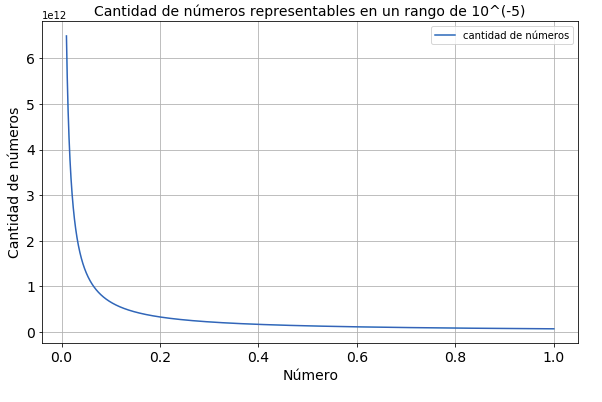
\includegraphics[scale=0.5]{precision_g}
    \end{figure}

\end{frame}

\begin{frame}{Comparaci\'on entre volatilidad impl\'icita y precio call con distintos ratios}

  \begin{figure}[t!]
    \centering
    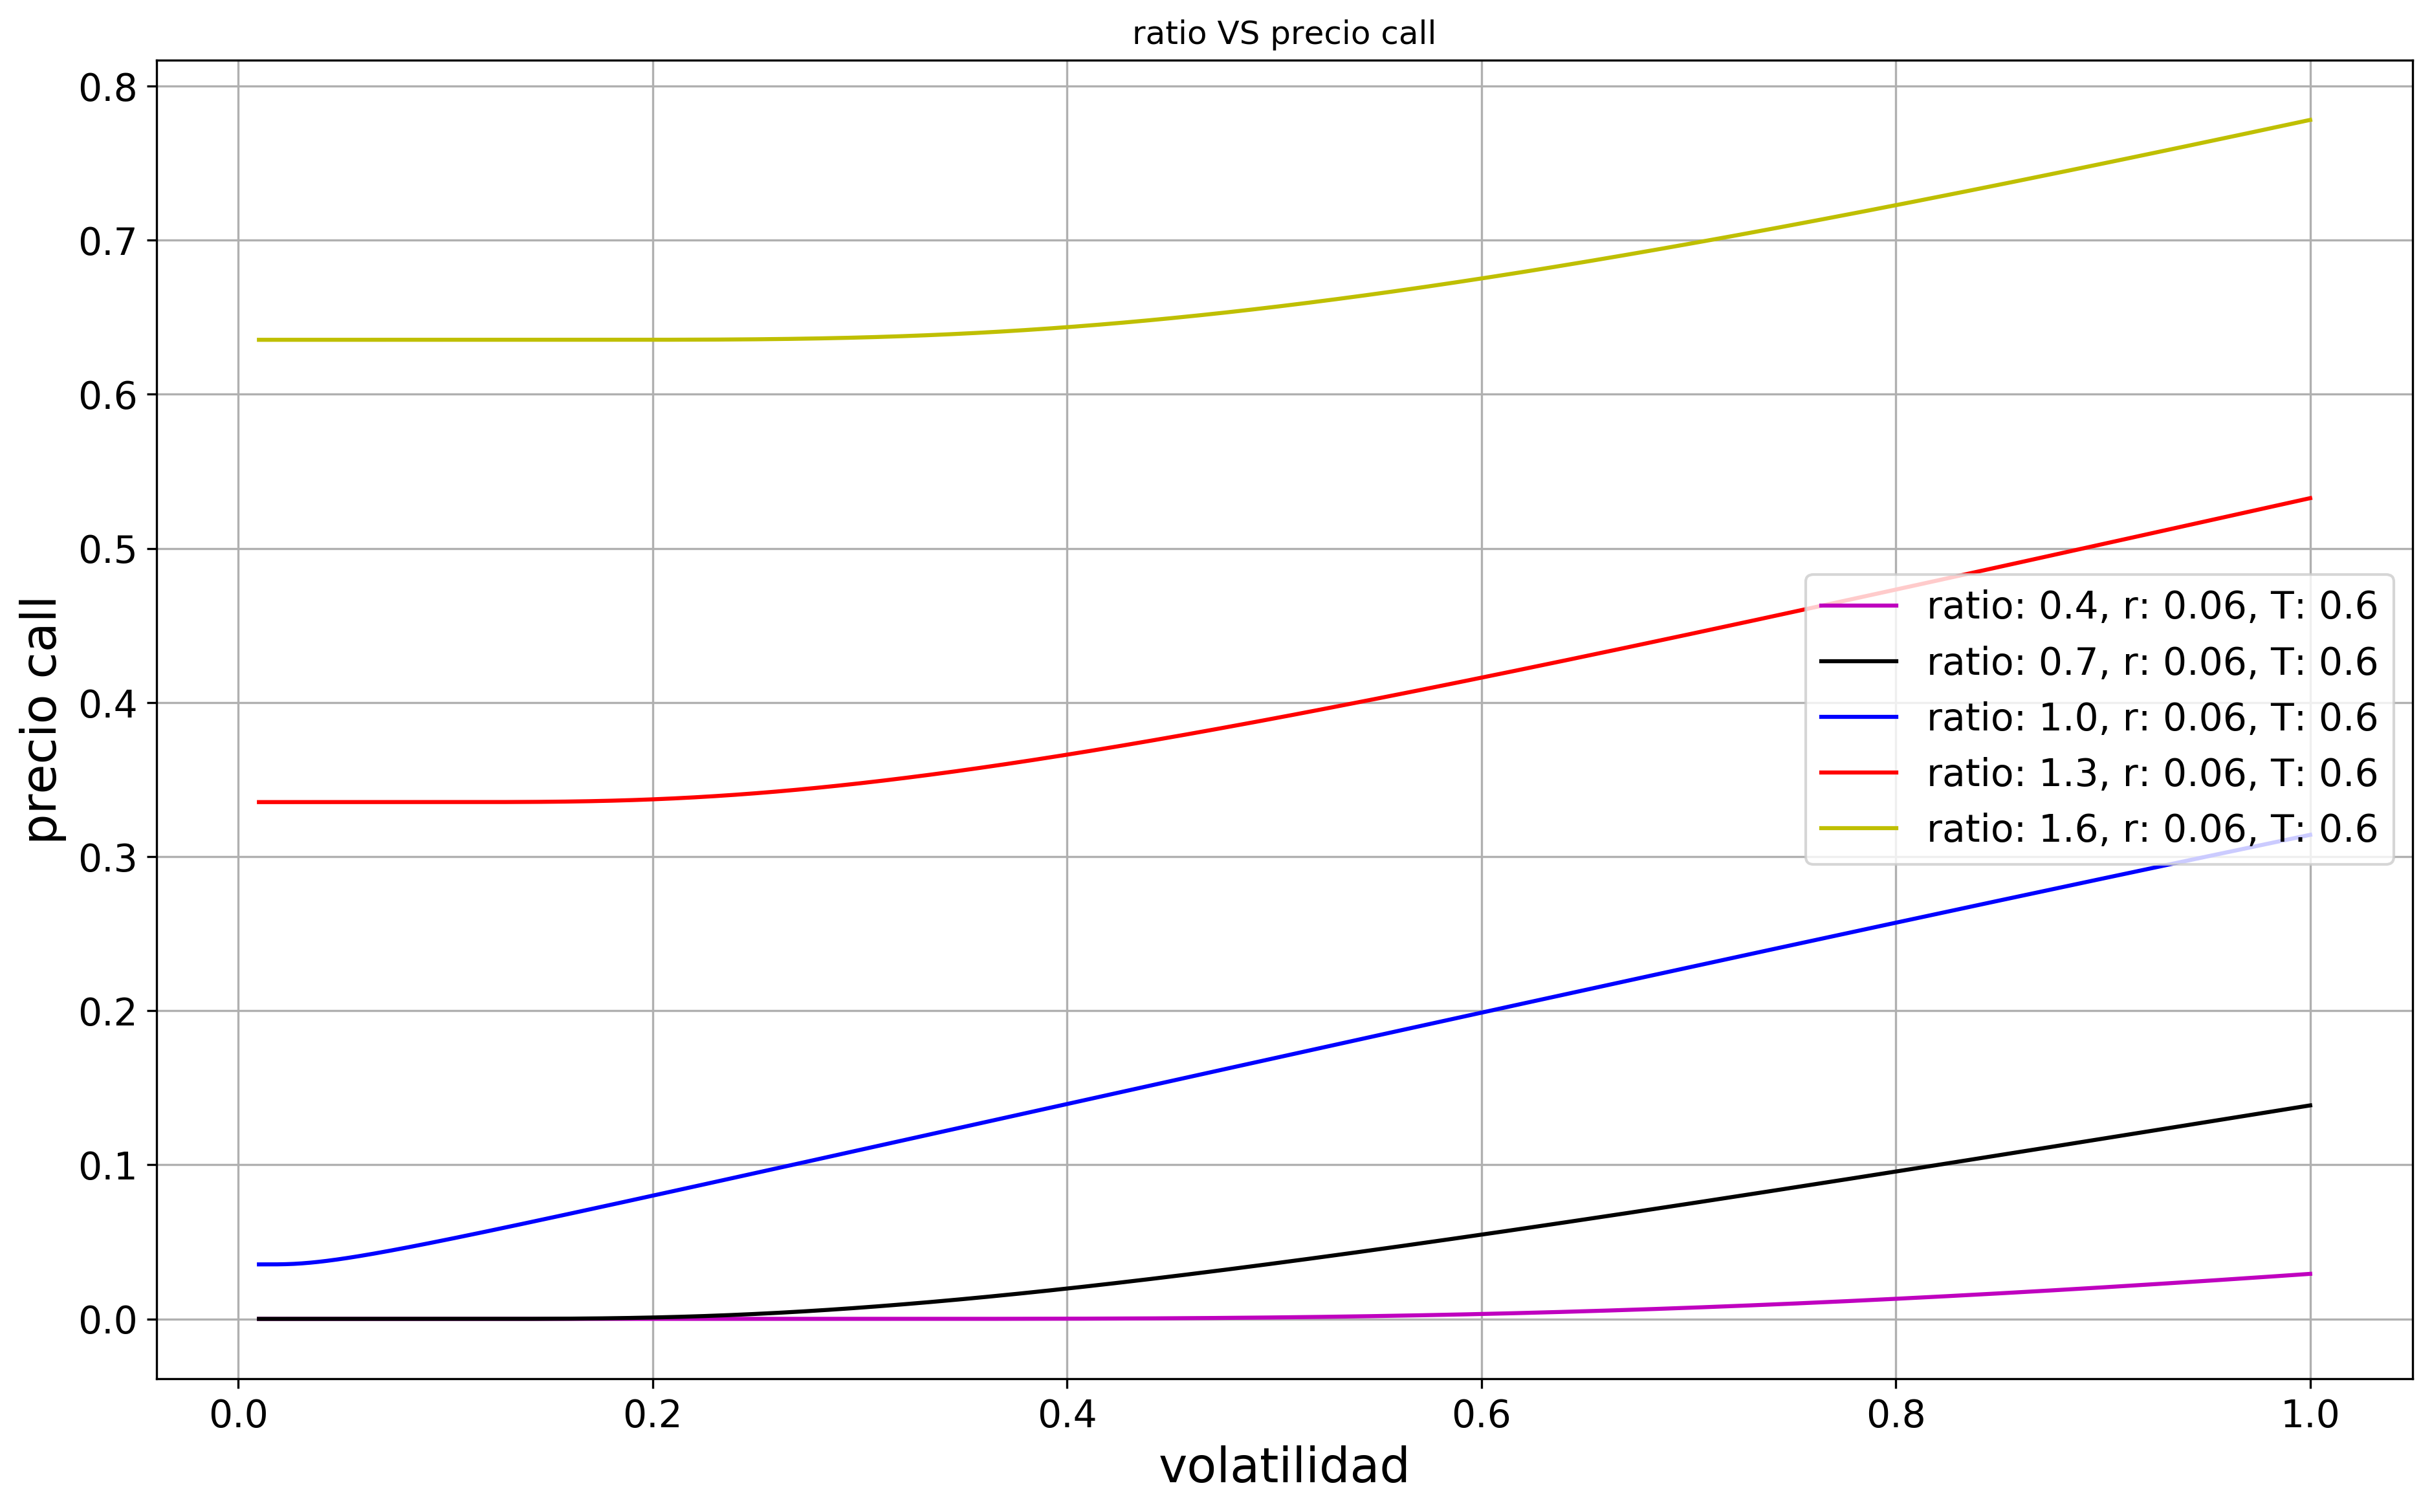
\includegraphics[width=11cm%, height=8cm
    ]{imagenes/ratio_v_call}
    
  \end{figure}

\end{frame}

\begin{frame}{Comparaci\'on entre volatilidad impl\'icita y precio call con distintas tasas de inter\'es}

  \begin{figure}[t!]
    \centering
    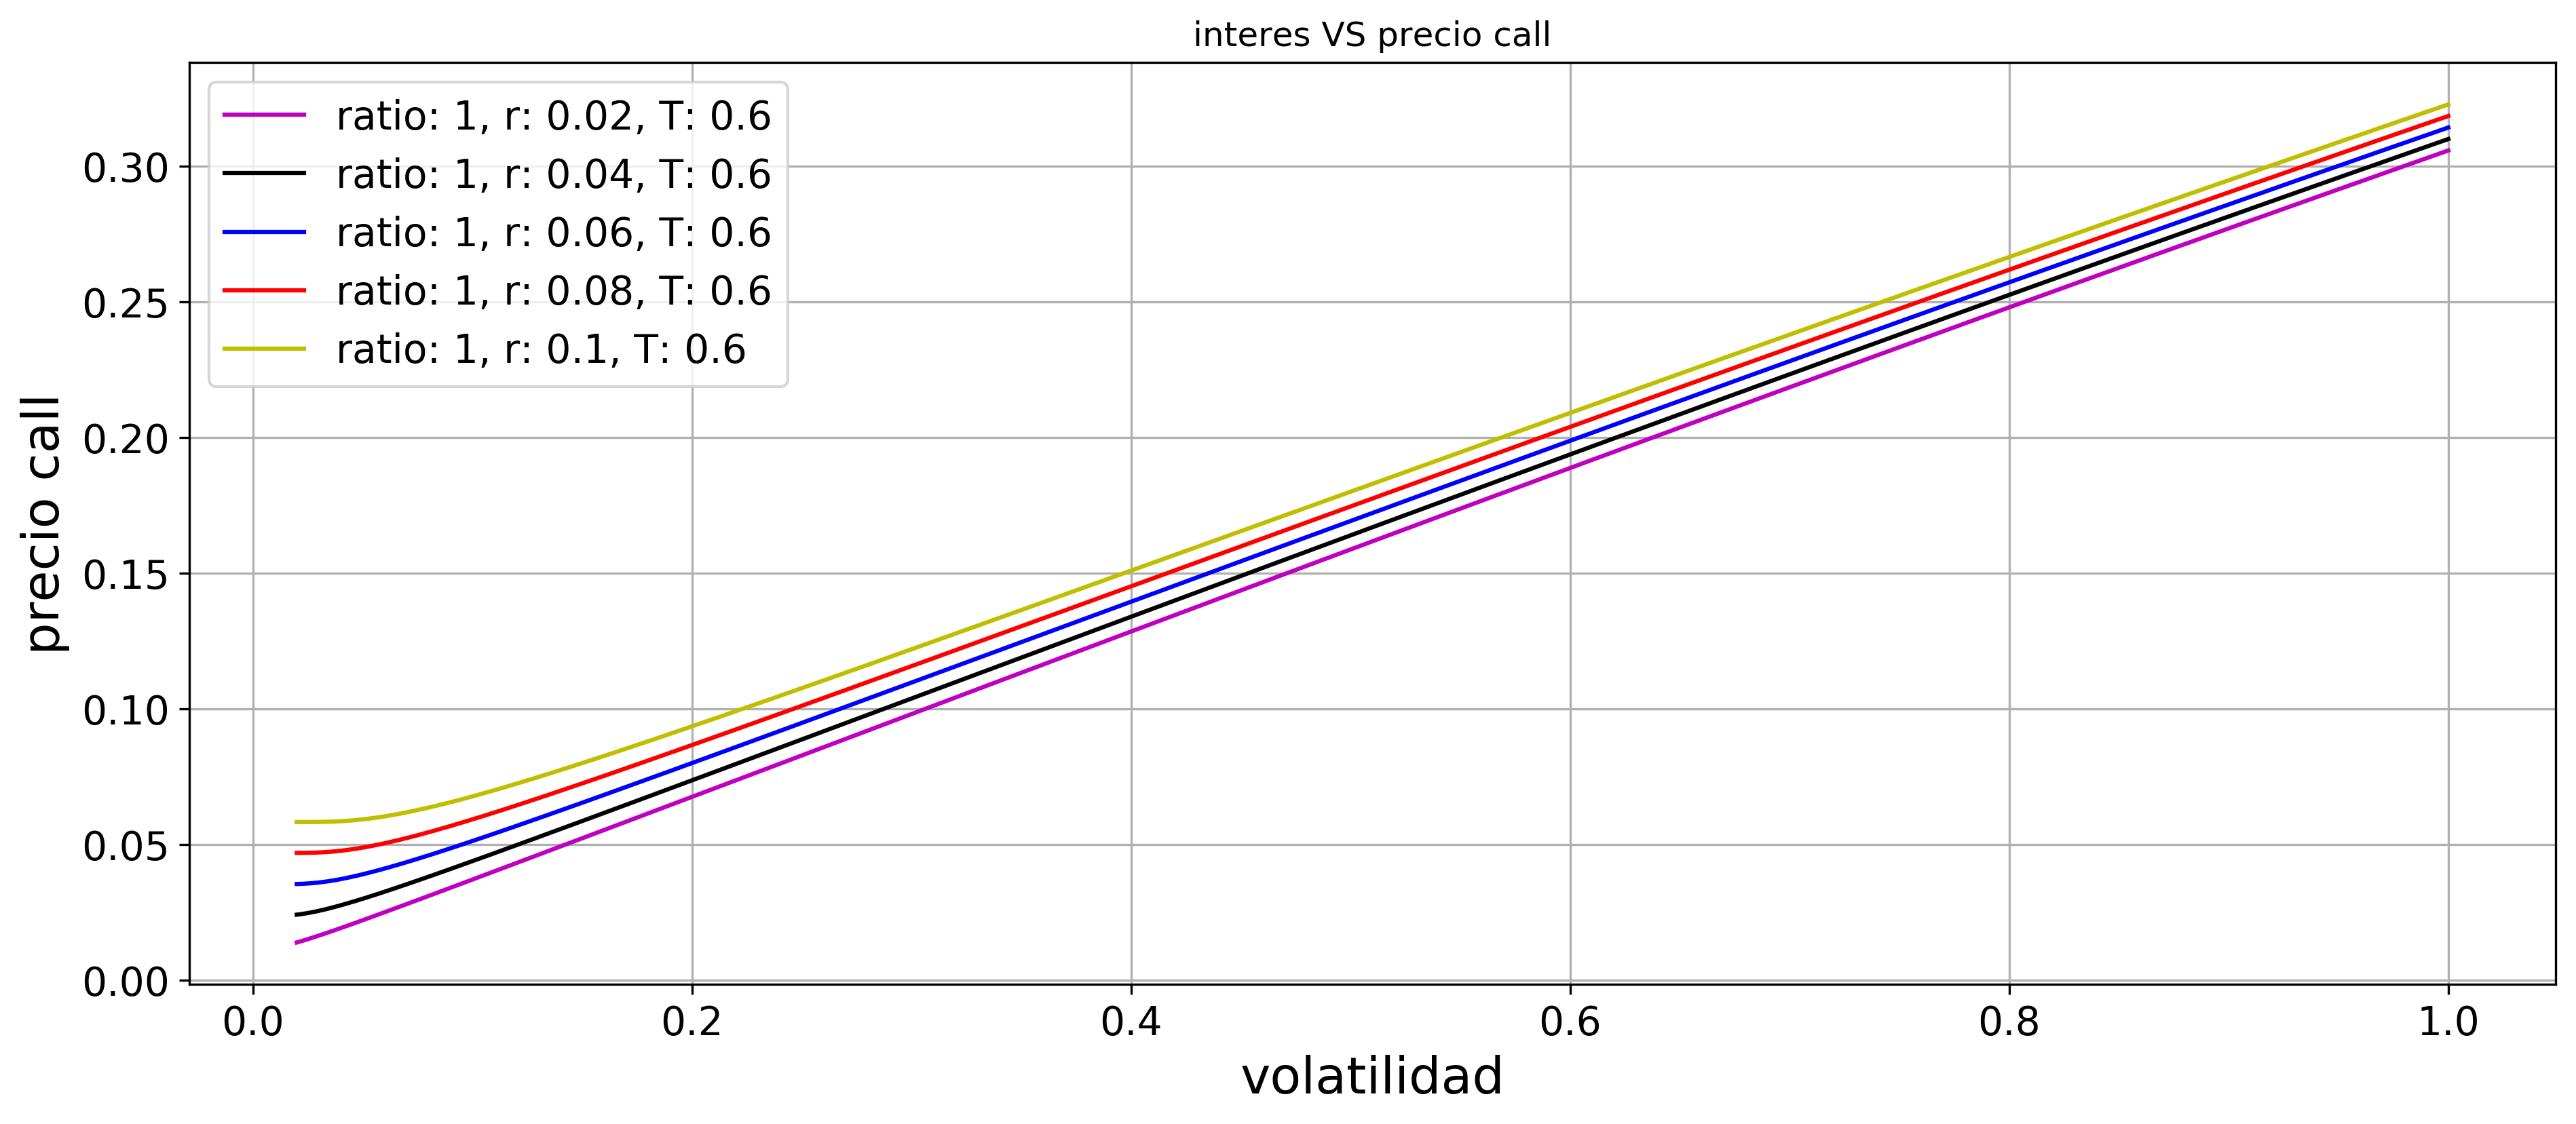
\includegraphics[width=11cm%, height=6cm
    ]{imagenes/interes_v_call}
  \end{figure}

\end{frame}



\begin{frame}{Comparaci\'on entre volatilidad impl\'icita y precio call con distintos tiempos de madurez}

  \begin{figure}[t!]
    \centering
    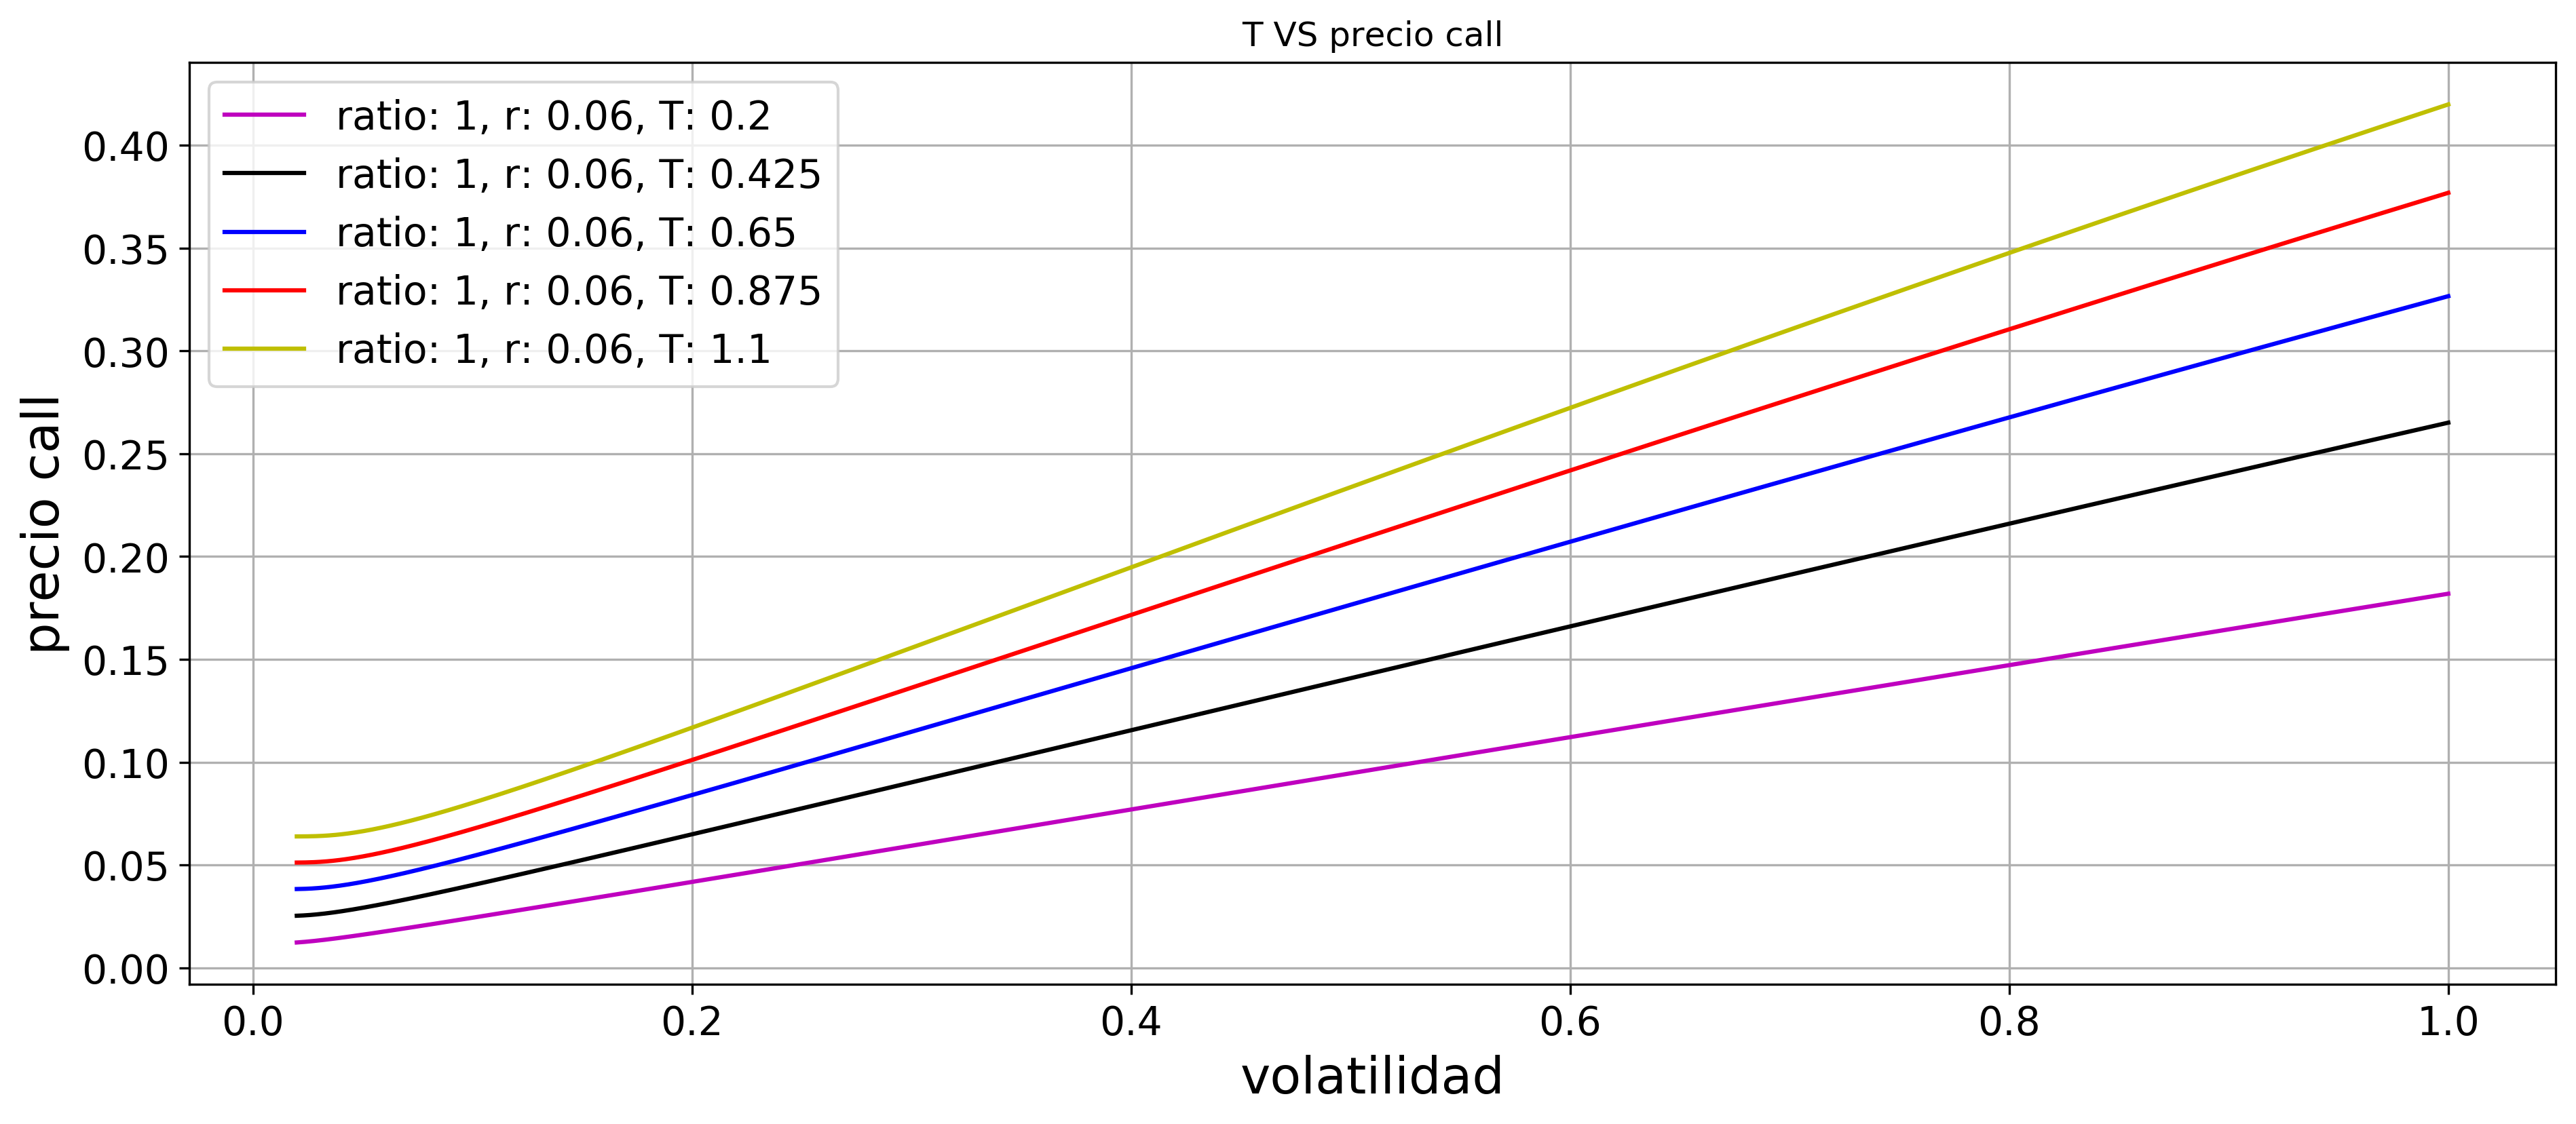
\includegraphics[width=11cm%, height=6cm
    ]{imagenes/T_v_call}
  \end{figure}
\end{frame}

\begin{frame}{Error de estimaci\'on en los M\'etodos Num\'ericos}

  \begin{block}{Impacto de la volatilidad impl\'icita con respecto al precio de la call}    
    \begin{itemize}
      \item Menos impacto en las opciones OTM.
      \item Menos impacto en las opciones cortas.
    \end{itemize}
  \end{block}

  \begin{block}{Error}
    En la pr\'actica se observa mas error en estimaci\'on sobre las opciones ITM con $\Phi(d_1)$ y
    $\Phi(d_2)$ cercanos a 1.
  \end{block}

\end{frame}

\begin{frame}{Problemas Num\'ericos en los M\'etodos de Bisecci\'on y Brent}
  Caso particular donde no se puede aplicar los m\'etodos num\'ericos.
  \begin{table}[!htbp]
    \centering
    \begin{tabular}{|ll|}
      \hline
      $c$: & $5.983489610184446$  \\ 
      $S$: & $15.752756180327959$  \\             % \cline{2-4} 
      $k$: & $10$   \\ % \cline{2-4} 
      $r$: & $0.09010364215460305$ \\               % \cline{2-4} 
      $T$: & $0.2590760904347537$  \\ \hline
    \end{tabular}
  \end{table}

  \begin{itemize}
    \item Si $\sigma = 0.01 \Rightarrow \Phi(d_1) = 1$, $\Phi(d_2) = 1$ y $g(\sigma) = 1.7763568394002505\times10^{-15}$.
    \item Si $\sigma = 0.11928197090875538 \Rightarrow \Phi(d_1) = 0.9999999999999986$, $\Phi(d_2) = 0.9999999999999982$ y $g(\sigma) = 0$.
  \end{itemize}

\end{frame}

\begin{frame}{Problemas Num\'ericos en los M\'etodos de Bisecci\'on y Brent}

    \begin{figure}[!tbp]
        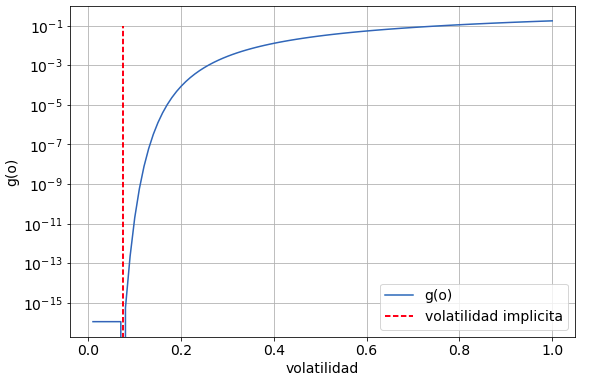
\includegraphics[scale=0.5]{g}
    \end{figure}

\end{frame}

\begin{frame}{Problemas Num\'ericos en los M\'etodos de Bisecci\'on y Brent}

    \begin{figure}[!tbp]
      \centering
      \begin{minipage}[b]{0.45\textwidth}
        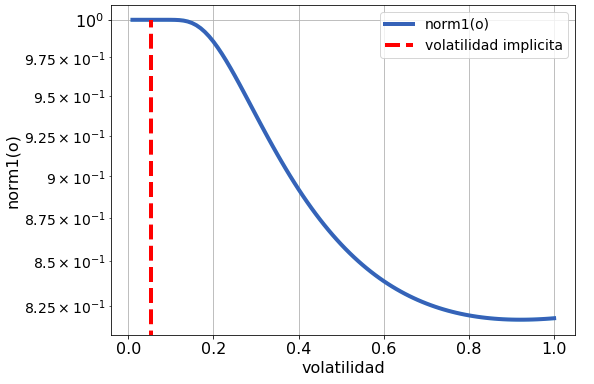
\includegraphics[width=\textwidth]{norm1.png}
        \caption{$\Phi(d_1)$}
      \end{minipage}
      \hfill
      \begin{minipage}[b]{0.45\textwidth}
        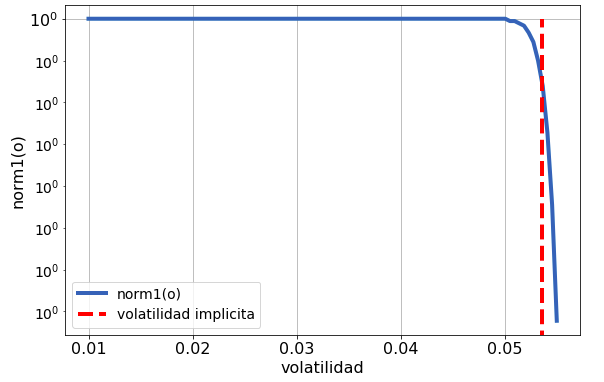
\includegraphics[width=\textwidth]{norm1_c.png}
        \caption{$\Phi(d_1)$}
      \end{minipage}
    \end{figure}

\end{frame}



\begin{frame}{Robustez y Tiempo de ejecuci\'on}
    
    Una vez entrenada la red (con un tiempo total de entrenamiento de 30 horas aproximadamente) en 
    GPU (GeForce GTX 1080/PCIe/SSE2), RAM (15.6 GiB). Comparamos su tiempo de ejecuci\'ion en 
    CPU (Intel(R) Core(TM) i5-8265U CPU @1.60GHz)

    \begin{table}[!htbp]
        \begin{center}
            \begin{tabular}{|l|l|l|l|l|}
                \hline
                 & Red Neuronal & Brent  &  Bisecci\'on  \\ \hline
                Tiempo (segundos)  & $7.34$  & $157.05$ & $318.31$   \\ \hline
                Robustez & Si  &  No & No \\ \hline
                  
            \end{tabular}
        \end{center}
    \end{table}

\end{frame}


\begin{frame}{Conclusiones}
  \begin{itemize}
    \item Importancia de la volatilidad imp\'icita.
    \item M\'etodos para la estimaci\'on volatidad imp\'icita.
  \end{itemize}
\end{frame}

\begin{frame}{Trabajos Futuros}

  \begin{itemize}
    \item Uso de GPU en la implementaci\'on de los modelos num\'ericos propuestos. 
    \item Soluciones para el problema num\'erico.
    \item Proponer otros modelos obtener la volatilidad impl\'icita.
  \end{itemize}

\end{frame}

\begin{frame}{?`Preguntas?}{}
\end{frame}

\end{document}